% ============================================================
%  BI-RADS Classification from Mammography Reports using
%  Kneser-Ney N-gram Language Models, Classical ML, and
%  Deep Recurrent Neural Networks
% ============================================================
\documentclass[11pt,a4paper]{article}

% --- Packages ---
\usepackage[margin=1in]{geometry}
\usepackage{setspace}
\onehalfspacing
\usepackage{amsmath,amssymb}
\usepackage{graphicx}
\usepackage{booktabs}
\usepackage{multirow}
\usepackage{array}
\usepackage{xcolor}
\usepackage{hyperref}
\usepackage{caption}
\usepackage{subcaption}
\usepackage{parskip}
\usepackage{enumitem}
\usepackage{tikz}
\usetikzlibrary{shapes.geometric, arrows.meta, positioning, fit, backgrounds}

\hypersetup{
    colorlinks=true,
    linkcolor=blue!60!black,
    citecolor=blue!60!black,
    urlcolor=blue!60!black
}

% --- Title ---
\title{%
  \textbf{BI-RADS Classification of Translated Mammography Reports:
  N-gram, Classical ML, and Deep Learning Approaches}
}

\author{%
  % TODO: author details
  % Replace this block with actual author names, affiliations, and emails.
  % Example format:
  % Author One$^{1}$, Author Two$^{1,2}$\\[4pt]
  % $^{1}$Department of ..., University of ..., City, Country\\
  % $^{2}$Department of ..., University of ..., City, Country\\
  % \texttt{author1@example.edu},\ \texttt{author2@example.edu}
  \textit{[Author details to be filled in]}
}

\date{}

\begin{document}

\maketitle
\thispagestyle{empty}

% ============================================================
\begin{abstract}
% ============================================================
Most mammography reports are written in the radiologist's native language,
which limits how much of the existing NLP tooling---overwhelmingly built and
tested on English---can be applied to them without extra work.
We study one way around this: translate the reports first, then classify.
Using a corpus of Portuguese mammography reports machine-translated into
English, we assign each report to one of the seven BI-RADS categories (0--6)
and compare three quite different modelling strategies on the same data:
Kneser-Ney smoothed N-gram language models scored via Maximum A-Posteriori
(MAP) inference, a sweep of classical bag-of-words classifiers, and three
recurrent neural network architectures.
To our knowledge, class-conditional Kneser-Ney models have not previously been
benchmarked on BI-RADS classification, so part of what we report here is simply
how well a fairly old-fashioned probabilistic approach holds up against newer
alternatives on the same leakage-free split.
After deduplicating an initial pool of 18{,}272 Portuguese reports and applying
a clinically aware preprocessing step, we are left with 9{,}179 reports, split
70/15/15 into train, validation, and test sets with class stratification.
All models are scored on the held-out test set using accuracy, macro-averaged
precision/recall/F1, and weighted F1.
TF-IDF features paired with a linear SVM gave the strongest overall result
(89.69\% accuracy, 89.99\% weighted F1), while an LSTM came out slightly ahead
on raw accuracy (90.27\%) with a comparable weighted F1 (89.88\%).
The Kneser-Ney bigram model, despite being by far the simplest of the three
families, reached 85.69\% accuracy and a macro F1 of 0.594 in just 4.66 seconds
over the entire test set---outperforming both the unigram and trigram variants.
We further provide an explainability analysis of the best deep learning model
(LSTM), combining per-class F1 attribution, ROC curves (macro AUC = 0.971),
prediction confidence profiling, and qualitative SHAP and LIME token-level
attributions. These analyses confirm that the LSTM's predictions are driven
primarily by measurement expressions, negation tokens, and laterality terms.
Taken together, the results suggest that a lightweight N-gram model is a
perfectly reasonable baseline for this kind of clinical text classification,
and that the gains from moving to discriminative classifiers or recurrent
networks are real but concentrated mainly in how well the minority BI-RADS
categories are handled.
\end{abstract}

% ============================================================
\section{Introduction}
% ============================================================

Breast cancer remains one of the most common cancers worldwide, and mammography
is still the frontline tool for catching it early.
When radiologists write up a mammogram, they summarise their impression using
the ACR BI-RADS (Breast Imaging Reporting and Data System) lexicon, a
seven-point scale (0 through 6) that also implies a recommended next step for
the patient~\cite{acr2013}.
Pulling that category back out of free-text reports by hand is slow, and
different readers do not always agree on borderline cases---both of which
become real problems once you are trying to audit a screening programme or run
a retrospective study at scale.

Automating this extraction is therefore a genuinely useful NLP problem, and it
gets harder once the reports are not in English.
Most of the world's radiology reporting happens in the local language of the
clinic, while the bulk of NLP research and tooling still targets English text.
One practical way to bridge that gap is to translate first and classify
second, which is the approach we take here: we translate Portuguese
mammography reports into English, run them through a clinically-aware
preprocessing step, and then train and compare three quite different families
of classifiers---N-gram language models, classical bag-of-words classifiers,
and recurrent neural networks---on the same data.

This paper's contributions are as follows.

\begin{enumerate}[label=(\roman*)]
  \item A clinically aware preprocessing pipeline for mammography reports that
        preserves negation cues, measurements, laterality terms, and
        clinical abbreviations while removing BI-RADS label leakage.
  \item A systematic benchmark of Kneser-Ney smoothed class-conditional
        N-gram language models (unigram, bigram, trigram) for BI-RADS
        classification, with MAP inference using class priors estimated from
        the training set.
  \item A ten-combination classical ML sweep (CountVectorizer/TF-IDF $\times$
        Naive Bayes/Logistic Regression/Linear SVM/Random Forest/XGBoost)
        with per-class analysis.
  \item Three end-to-end deep learning models (RNN, LSTM, BiLSTM) with
        shared embedding and recurrent architecture, trained with early stopping
        and evaluated on an identical test split.
  \item A comprehensive comparison across all three tiers on the same
        stratified 70/15/15 split, enabling fair head-to-head ranking.
  \item An explainability analysis of the best deep learning model (LSTM)
        covering per-class F1 attribution, macro-averaged ROC curves
        (AUC = 0.971), prediction confidence calibration, and qualitative
        SHAP and LIME token-level attributions, confirming that measurement
        expressions, negation tokens, and laterality terms are the
        primary drivers of LSTM predictions.
\end{enumerate}

% ============================================================
\section{Preliminaries / Background}
% ============================================================

\subsection{BI-RADS Assessment Categories}

The ACR BI-RADS system defines seven assessment categories for mammographic
screening reports~\cite{acr2013}:

\begin{itemize}
  \item \textbf{Category 0}: Incomplete --- additional imaging needed.
  \item \textbf{Category 1}: Negative --- no significant finding.
  \item \textbf{Category 2}: Benign finding --- no malignancy.
  \item \textbf{Category 3}: Probably benign --- short-interval follow-up.
  \item \textbf{Category 4}: Suspicious --- biopsy should be considered.
  \item \textbf{Category 5}: Highly suggestive of malignancy.
  \item \textbf{Category 6}: Known biopsy-proven malignancy.
\end{itemize}

Category~2 (benign) dominates most screening datasets because the majority of
mammograms are normal or benign; categories 5 and 6 are rare.
This severe class imbalance is a defining challenge for BI-RADS classification.

\subsection{N-gram Language Models and Kneser-Ney Smoothing}

A class-conditional N-gram language model assigns a log-probability to a
document $\mathbf{w} = (w_1, \ldots, w_T)$ under class $c$:

\begin{equation}
  \log P(\mathbf{w} \mid c)
  = \sum_{t=1}^{T} \log P_c(w_t \mid w_{t-N+1}^{t-1})
\end{equation}

For MAP classification, the predicted class is
$\hat{c} = \arg\max_c \bigl[\log P(\mathbf{w}\mid c) + \log P(c)\bigr]$,
where $P(c)$ is the empirical class prior on the training set.

Kneser-Ney smoothing \cite{kneser1995improved} is the interpolated extension
used in this work.
For bigrams it is:

\begin{equation}
  P_{\text{KN}}(w \mid h) =
    \frac{\max(C(h,w) - D, 0)}{C(h)}
    + \lambda(h)\,P_{\text{continuation}}(w)
\end{equation}

where $D$ is an absolute discount estimated from counts-of-counts
($D = n_1 / (n_1 + 2n_2)$), $\lambda(h)$ is the interpolation weight,
and $P_{\text{continuation}}(w) \propto |\{h' : C(h',w) > 0\}|$ measures the
novelty of $w$ as a right-continuation across all contexts. This absolute-discounting
formulation, along with its trigram extension, follows the smoothing family
evaluated extensively by Chen and Goodman~\cite{chen1998evaluation}.

For trigrams, Kneser-Ney recursively backs off to the smoothed bigram estimate.
For words unseen in the vocabulary (out-of-vocabulary tokens), Laplace-smoothed
unigrams serve as the ultimate back-off.

\subsection{TF-IDF and Count Vectorizer Features}

Classical discriminative classifiers operate on bag-of-words (BoW) feature
vectors.
Two feature representations are used:
\begin{itemize}
  \item \textbf{CountVectorizer}: Raw term-frequency counts over a
        vocabulary of the top $k$ tokens by frequency.
  \item \textbf{TF-IDF} (Term Frequency--Inverse Document Frequency):
        Downweights terms that are uniformly common across classes,
        amplifying class-discriminative terms, following the classical
        term-weighting formulation of Salton and Buckley~\cite{salton1988term}.
\end{itemize}

Both representations are fit exclusively on the training split to prevent
data leakage.

\subsection{Recurrent Neural Networks for Text Classification}

Recurrent neural networks (RNNs) process sequences token-by-token, maintaining
a hidden state $h_t = f(W_h h_{t-1} + W_x x_t)$.
Long Short-Term Memory (LSTM) networks~\cite{hochreiter1997long} augment the
basic RNN with cell-state gating (input, forget, output gates) to capture
long-range dependencies while mitigating vanishing gradients.
Bidirectional LSTMs (BiLSTMs)~\cite{schuster1997bidirectional} concatenate
forward and backward hidden states, enabling each position to attend to both
preceding and following context---a useful property for sentence-final negations
and result summaries common in radiology reports.

All three architectures---RNN, LSTM, and BiLSTM---share the same overall
shape: an embedding layer feeds into the recurrent block, which is followed
by global average pooling, a dense ReLU layer, dropout, and finally a softmax
output.

% ============================================================
\section{Related Works}
% ============================================================

Interest in automatically classifying radiology reports has grown steadily
over the last decade, for fairly obvious reasons: the reports already exist in
large numbers, and manually coding them does not scale.
Hassanpour and Langlotz~\cite{hassanpour2017information} showed early on that
both rule-based and learned methods could pull structured information out of
radiology text with reasonable accuracy. In a related but distinct line of
work, Yala et al.~\cite{yala2019deep} used an image-based deep learning model
on the mammogram pixels themselves (rather than the report text) to improve
breast-cancer risk prediction, illustrating the broader push toward deep
learning across the mammography workflow; closer to our own report-classification
setting, Karimi et al.~\cite{karimi2017automatic} directly compared deep
learning and conventional classifiers for autocoding radiology reports.
Negation handling turns out to matter a great deal in this domain---Peng et
al.~\cite{peng2018negbio} make this point well with their NegBio tool, and it
is a large part of why our own preprocessing goes out of its way to preserve
negation cues rather than stripping them out as generic stopwords.

N-gram language models are, admittedly, an old idea, but they have stuck
around in clinical NLP precisely because they are simple, fast, and easy to
inspect \cite{friedman2004natural}. Kneser-Ney smoothing in particular is still
regarded as one of the more reliable ways to generalise from sparse counts
\cite{chen1998evaluation}, which made it an appealing choice here given how few
training examples exist for BI-RADS categories 5 and 6.

Transformer models such as ClinicalBERT \cite{alsentzer2019publicly} and
BioMedBERT now define the state of the art on many clinical NLP benchmarks,
but they come with real costs---GPU infrastructure, larger fine-tuning
datasets, longer iteration cycles---that are not always available, especially
outside well-resourced hospital systems. We see the models compared in this
paper less as competitors to transformers and more as a lower-cost baseline
worth establishing first.

Work specifically on Portuguese-language clinical text is comparatively rare.
Nassif et al.~\cite{nassif2012extracting} built the first BI-RADS feature
parser for Portuguese free text, but it targets feature-level extraction
rather than full BI-RADS category classification and does not compare
multiple model families head to head under one evaluation protocol, which is
part of the gap this paper tries to fill. More broadly, our translate-then-classify
setup follows the strategy examined by Artetxe et al.~\cite{artetxe2023revisiting},
who show that translating text into a high-resource language before applying
a monolingual classifier (``translate-test'') can be competitive with training
multilingual models directly, and echoes the translation-based cross-lingual
transfer strategies for clinical text explored by Papaioannou et
al.~\cite{papaioannou2022cross} for non-English clinical phenotyping.

% ============================================================
\section{Problem Statement}
% ============================================================

We work with a corpus of free-text Portuguese mammography reports, each
associated with a ground-truth BI-RADS category label in $\{0, 1, 2, 3, 4,
5, 6\}$, together with machine-translated English versions of each report,
partitioned into a class-stratified 70/15/15 train/validation/test split of
$n = 9{,}179$ reports. The objective is to construct a set of NLP
models----(i) class-conditional N-gram language models with Kneser-Ney
smoothing and MAP inference, (ii) bag-of-words discriminative classifiers,
and (iii) deep recurrent neural networks---to automatically predict the
BI-RADS category of a mammography report from its translated and
preprocessed text, and to compare their performance under a unified
evaluation protocol using accuracy, macro-averaged F1, and weighted F1 on
the held-out test set. Because macro and weighted F1 can rank models very
differently under severe class imbalance, we report both throughout,
following the guidance on evaluation-measure choice for imbalanced
classification tasks given by Sokolova and
Lapalme~\cite{sokolova2009systematic} and by Saito and
Rehmsmeier~\cite{saito2015precision}.

Figure~\ref{fig:pipeline} illustrates the end-to-end system architecture.

\begin{figure}[h!]
\centering
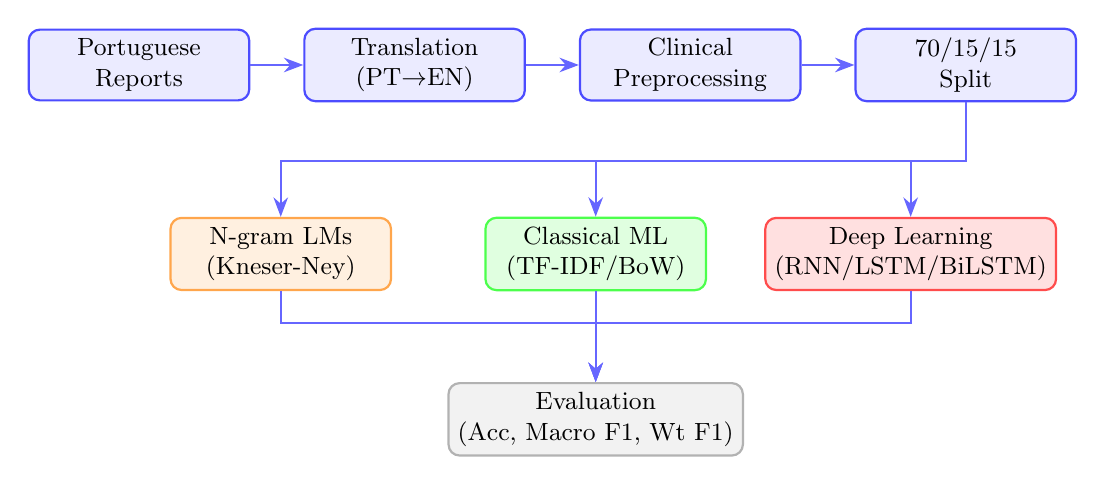
\begin{tikzpicture}[
  box/.style={
    rectangle, rounded corners=4pt,
    draw=blue!70, fill=blue!8, thick,
    minimum width=2.8cm, minimum height=0.85cm,
    align=center, font=\small
  },
  arrow/.style={-{Stealth[length=7pt]}, thick, blue!60}
]

% ---- Top row ----
\node[box] (raw)   at (0,0)     {Portuguese\\Reports};
\node[box] (trans) at (3.5,0)   {Translation\\(PT$\to$EN)};
\node[box] (pre)   at (7.0,0)   {Clinical\\Preprocessing};
\node[box] (split) at (10.5,0)  {70/15/15\\Split};

% ---- Model row ----
\node[box, fill=orange!12, draw=orange!70]
             (ngram) at (1.8,-2.4) {N-gram LMs\\(Kneser-Ney)};
\node[box, fill=green!12, draw=green!70]
             (ml)    at (5.8,-2.4) {Classical ML\\(TF-IDF/BoW)};
\node[box, fill=red!12, draw=red!70]
             (dl)    at (9.8,-2.4) {Deep Learning\\(RNN/LSTM/BiLSTM)};

% ---- Evaluation row ----
\node[box, fill=gray!10, draw=gray!60]
             (eval)  at (5.8,-4.5) {Evaluation\\(Acc, Macro F1, Wt F1)};

% ---- Arrows ----
\draw[arrow] (raw)   -- (trans);
\draw[arrow] (trans) -- (pre);
\draw[arrow] (pre)   -- (split);

\draw[arrow] (split.south) |- ++(0,-0.75) -| (ngram.north);
\draw[arrow] (split.south) |- ++(0,-0.75) -| (ml.north);
\draw[arrow] (split.south) |- ++(0,-0.75) -| (dl.north);

\draw[arrow] (ngram.south) |- ++(0,-0.4) -| (eval.north);
\draw[arrow] (ml.south)    -- (eval.north);
\draw[arrow] (dl.south)    |- ++(0,-0.4) -| (eval.north);

\end{tikzpicture}
\caption{End-to-end pipeline for BI-RADS classification from translated
         mammography reports.}
\label{fig:pipeline}
\end{figure}

% ============================================================
\section{Proposed Work}
% ============================================================

This section describes the full experimental pipeline in four stages: data
collection and quality auditing, clinical-domain-aware preprocessing, model
construction across the three families introduced above (N-gram language
models, classical ML, and deep learning), and the experimental protocol used
to compare them. All stages operate on the same stratified 70/15/15 split
described in the Problem Statement and are implemented to be fully
reproducible.

\subsection{Data Collection}

We start from $18{,}272$ Portuguese-language mammography reports, each labelled
with one of the seven BI-RADS categories.\footnote{Raw data, preprocessing
scripts, notebooks, and all intermediate artefacts referenced in this section
are provided in the accompanying code repository for reproducibility.}
An initial audit turned up no missing values and no empty reports, but a
surprising number of exact-text duplicates---$9{,}093$ of them. After removing
these and running the reports through the preprocessing pipeline described
below, $9{,}179$ unique reports remain for modelling.

As is typical for screening data, the raw class distribution is heavily
skewed: Category~2 (benign) alone accounts for 15{,}968 of the 18{,}272 raw
records (87.4\%), whereas Categories~5 and~6 together make up only 74 reports
(0.4\%). This imbalance shapes a lot of what follows, particularly the
macro-F1 results in Section~\ref{sec:results}.

Every report is machine-translated from Portuguese into English using an automated translation service. A manual spot-check of 50 randomly sampled reports was conducted to assess the preservation of clinical terminology, negation, measurement expressions, and laterality (left/right/bilateral) during translation. No critical translation errors were identified in the sampled reports.

\subsection{Preprocessing}

Preprocessing is applied uniformly across the train, validation, and test
splits, and is deliberately clinical-domain-aware rather than generic.
Figure~\ref{fig:preprocessing_pipeline} summarises the full sequence, from
the raw Portuguese reports through to model-ready English text.

\begin{figure}[h!]
\centering
\includegraphics[width=\textwidth]{figures/preprocessing_pipeline.png}
\caption{End-to-end preprocessing pipeline: data quality auditing, target
         leakage detection, Portuguese-to-English translation, translation
         validation, text normalisation, domain-aware processing, and a
         final post-processing quality check.}
\label{fig:preprocessing_pipeline}
\end{figure}

Each stage is described in more detail below:

\paragraph{Clinical abbreviation expansion.}
Common radiology abbreviations (e.g.\ \texttt{yo}$\to$\textit{year old},
\texttt{r/o}$\to$\textit{rule out}, \texttt{bilat}$\to$\textit{bilateral})
are expanded using a curated dictionary applied as whole-word, case-insensitive
replacements.

\paragraph{Negation normalisation.}
Stopwords are intentionally \emph{not} removed.
Negation tokens (``no'', ``not'', ``without'', ``denies'', ``unremarkable'',
etc.) carry critical clinical meaning and must be preserved.

\paragraph{Measurement preservation.}
A regular expression pattern protects measurement spans
(e.g.\ ``2.5~cm'', ``3$\times$2$\times$1.5~cm'') from punctuation stripping
by using an internal placeholder.

\paragraph{Laterality preservation.}
Laterality abbreviations (\texttt{rt}, \texttt{lt}, \texttt{b/l}) are expanded
to canonical forms (\textit{right}, \textit{left}, \textit{bilateral}).

\paragraph{BI-RADS leakage removal.}
All explicit mentions of the BI-RADS category (``BI-RADS~3'', ``Category~4'',
etc.) and conclusive diagnosis terms (``malignant'', ``benign'',
``biopsy-proven'') are removed from the report text to prevent trivial
label leakage.
A post-cleaning quality check found that 181 reports still contained residual
partial matches (e.g.\ a fragment of a removed phrase); rather than discard
these outright, we flagged them and kept them in the dataset to avoid losing
data unnecessarily.

\paragraph{Dataset splits.}
The processed dataset ($9{,}179$ records) is split with stratification:

\begin{table}[h!]
\centering
\caption{Stratified data split statistics.}
\label{tab:splits}
\begin{tabular}{lcccccccc}
\toprule
\textbf{Split} & \textbf{Total} &
  \textbf{BI-0} & \textbf{BI-1} & \textbf{BI-2} &
  \textbf{BI-3} & \textbf{BI-4} & \textbf{BI-5} & \textbf{BI-6} \\
\midrule
Train      & 6{,}425 & 423 & 176 & 5{,}126 & 498 & 150 & 20 & 32 \\
Validation & 1{,}377 & 91  & 38  & 1{,}098 & 107 & 32  & 4  & 7  \\
Test       & 1{,}377 & 91  & 38  & 1{,}099 & 106 & 32  & 5  & 6  \\
\bottomrule
\end{tabular}
\end{table}

Reports average 53.91 words (raw) and 52.55 words (processed), ranging from
20 to 234 words.

\subsection{Model Construction}
\label{sec:model_construction}

We constructed three complementary families of models to investigate probabilistic, conventional machine-learning, and deep-learning approaches for BI-RADS classification.

\subsubsection{N-gram Language Models (Probabilistic)}

For each of the seven BI-RADS categories, a separate class-conditional Kneser--Ney language model was constructed.

\textbf{Tokenisation.}
Reports were lowercased and tokenised using a regular-expression tokenizer with the pattern
\texttt{[a-z0-9]+(?:[./-]\allowbreak[a-z0-9]+)*}.
This pattern preserves hyphenated terms, slash-based constructions, and decimal measurements as individual tokens. No stopword removal was applied.

\textbf{Closed Vocabulary and OOV Handling.}
A shared closed vocabulary was constructed exclusively from the training partition by retaining tokens occurring at least twice ($f \geq 2$), resulting in $|\mathcal{V}| = 1{,}592$ token types. The vocabulary was fixed after construction and was not expanded using validation or test data. Tokens absent from the retained training vocabulary were treated as out-of-vocabulary (OOV) tokens and mapped to a dedicated \texttt{<UNK>} token. The observed OOV rates remained below  1\% across the training, validation, and test partitions.

\textbf{Smoothing and Back-off.}
The Kneser--Ney absolute discount parameter $D$ was estimated from counts-of-counts as

$$
D = \frac{n_1}{n_1 + 2n_2},
$$

where $n_1$ and $n_2$ denote the numbers of n-grams with frequencies one and two, respectively, following the counts-of-counts discount estimator described in~\cite{chen1998evaluation}. Discount estimation was performed separately for bigram and trigram models within each BI-RADS class. For higher-order models, unseen contexts were resolved through a hierarchical back-off mechanism from trigram probabilities to bigram probabilities, followed by the Kneser--Ney continuation probability and, where required, a Laplace-smoothed unigram probability.

\textbf{Inference.}
Given a tokenised test report represented by $\mathbf{w}$, each class-conditional language model estimates the report likelihood $P(\mathbf{w}\mid c)$. Classification is performed using a maximum a posteriori (MAP) decision rule:

$$
\hat{c}
=
\arg\max_c
\left[
\log P(\mathbf{w}\mid c)
+
\log \hat{P}(c)
\right],
$$

where $\hat{P}(c)$ denotes the empirical class prior estimated from the training partition. Independent class-conditional models were constructed and evaluated for unigram, bigram, and trigram orders ($n \in {1,2,3}$).

Figure~\ref{fig:ngram_pipeline} summarises the class-wise language-model construction and MAP-based classification procedure.


\begin{figure}[h!]
\centering
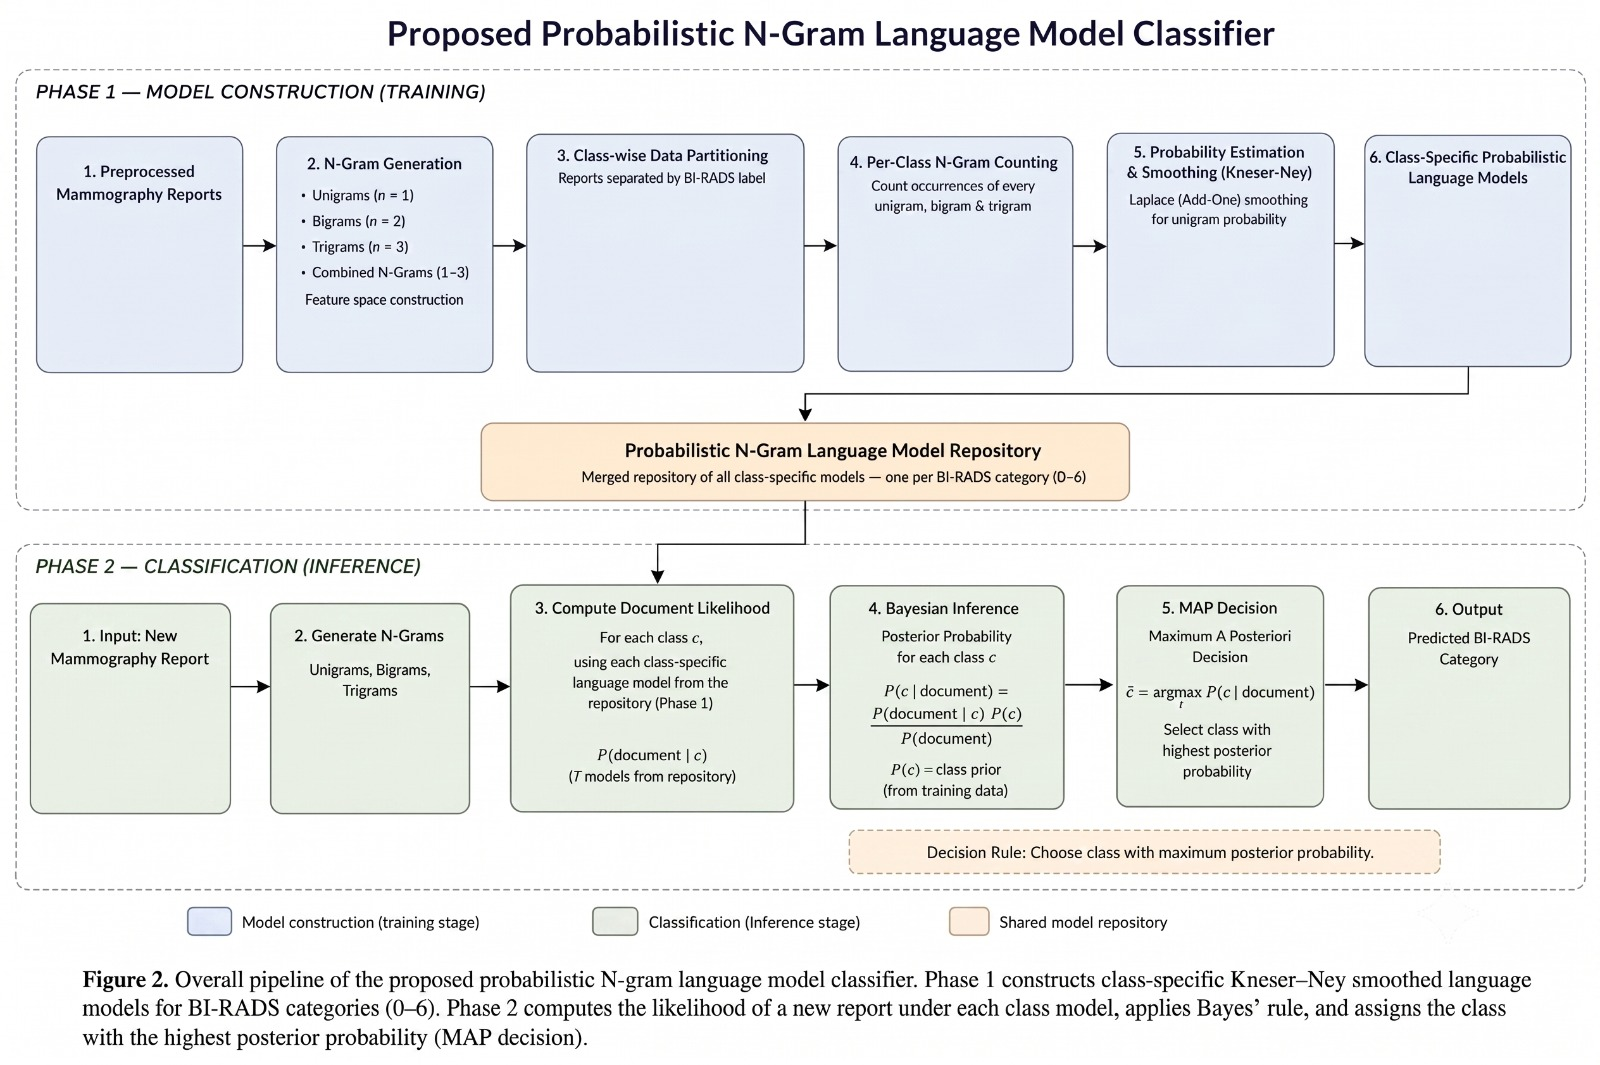
\includegraphics[width=\textwidth]{figures/ngram_classifier.jpeg}
\caption{Overall pipeline of the two-phase N-gram model classification approach. Phase 1 (top) constructs class-specific Kneser-Ney smoothed language
models for BI-RADS categories (0-6). Phase 2 (bottom) computes the likelihood of a new report under each class model, applies Bayes' rule, and assigns the class
with the highest posterior probability (MAP decision).}
\label{fig:ngram_pipeline}
\end{figure}

\subsubsection{Classical Machine Learning}

For the classical ML tier, we train every combination of two feature
extractors and five model families---ten combinations in total.

\textbf{Feature extraction:}
\begin{itemize}
  \item \textbf{CountVectorizer}: top-$k$ unigram bag-of-words counts
        (fit on training set only).
  \item \textbf{TF-IDF}: $\ell_2$-normalised TF-IDF scores over the same
        vocabulary, following Salton and Buckley~\cite{salton1988term}.
\end{itemize}

\textbf{Models:}
\begin{enumerate}
  \item Multinomial Naive Bayes, using the multinomial event model compared
        by McCallum and Nigam~\cite{mccallum1998naive}
  \item Logistic Regression with $\ell_2$ penalty, \texttt{class\_weight=balanced},
        \texttt{max\_iter=1000}
  \item Linear SVM (\texttt{LinearSVC}), \texttt{class\_weight=balanced},
        following the text-categorisation formulation of
        Joachims~\cite{joachims1998text}
  \item Random Forest, 300 trees, \texttt{class\_weight=balanced}, as
        introduced by Breiman~\cite{breiman2001random}
  \item XGBoost~\cite{chen2016xgboost}
\end{enumerate}

All models are trained on $X_{\text{train}}$ and evaluated on $X_{\text{val}}$
and $X_{\text{test}}$ using features extracted with the \emph{training-fit}
vectorizer.

\subsubsection{Deep Learning --- RNN, LSTM, BiLSTM}

For the deep learning tier, we train three recurrent architectures on the
same splits used throughout the paper.

\textbf{Tokenisation.}
Keras \texttt{Tokenizer} with \texttt{vocab\_size=20{,}000}, \texttt{<OOV>}
token, padded/truncated to \texttt{max\_len=300} tokens.

\textbf{Architecture.} All three models share the same skeleton: a 128-dimensional
embedding layer, a 128-unit recurrent block, global average pooling, a
64-unit dense ReLU layer, dropout at a rate of 0.4, and a 7-way softmax
output. The embedding layer is trained end-to-end from a random initialisation
rather than initialised from pre-trained vectors such as word2vec~\cite{mikolov2013efficient}
or GloVe~\cite{pennington2014glove}; we return to this design choice, and the
possibility of using pre-trained embeddings, in Section~\ref{sec:strengths}.

The recurrent block differs per architecture: the RNN model uses
\texttt{SimpleRNN(128)}, the LSTM model uses \texttt{LSTM(128)}, and the
BiLSTM model uses \texttt{Bidirectional(LSTM(128))}.

\textbf{Training hyperparameters.}
Adam optimiser ($\text{lr} = 10^{-3}$), categorical cross-entropy loss,
batch size 32, up to 30 epochs with early stopping (patience = 4)
on validation loss.
Best checkpoint (lowest validation loss) is restored before test evaluation.
Model weights are saved under \texttt{models/deep\_learning/} as
\texttt{rnn\_best.keras}, \texttt{lstm\_best.keras}, \texttt{bilstm\_best.keras}.

\subsection{Experiments}

\subsubsection{Setup}

The data split follows the stratified 70/15/15 train/validation/test
partition described in Table~\ref{tab:splits}, and hyperparameters for each
model family are as described in Section~\ref{sec:model_construction}.
Evaluation is carried out on the test-set predictions using Accuracy, Macro
Precision, Macro Recall, Macro F1, and Weighted F1. Macro averaging treats
each class equally, which is critical for surfacing minority-BI-RADS
performance, whereas weighted averaging reflects real-world class frequency;
this macro/weighted distinction, and its importance under class imbalance, is
discussed at length by Sokolova and Lapalme~\cite{sokolova2009systematic}.
All final numbers reported below come from the held-out test set of
1{,}377 reports.

\subsubsection{Results}
\label{sec:results}

\paragraph{N-gram model comparison (validation set).}

Table~\ref{tab:ngram_val} reports validation-set performance for all three
N-gram orders.

\begin{table}[h!]
\centering
\caption{N-gram order comparison on the validation set.}
\label{tab:ngram_val}
\begin{tabular}{lcccccc}
\toprule
\textbf{Model} & \textbf{Acc.} &
  \textbf{P\textsubscript{mac}} & \textbf{R\textsubscript{mac}} &
  \textbf{F1\textsubscript{mac}} & \textbf{F1\textsubscript{wt}} &
  \textbf{Infer.\ (s)} \\
\midrule
Unigram & 0.769 & 0.394 & 0.433 & 0.384 & 0.784 & 0.862 \\
Bigram  & 0.853 & 0.626 & 0.563 & \textbf{0.585} & 0.852 & 3.238 \\
Trigram & 0.847 & 0.614 & 0.540 & 0.552 & 0.844 & 7.471 \\
\bottomrule
\end{tabular}
\end{table}

The Bigram model achieves the best validation Macro F1 (0.585) and
accuracy (85.3\%), leading to its selection as the final N-gram model.

\paragraph{N-gram selected model --- test set.}

Table~\ref{tab:ngram_test} shows the Kneser-Ney Bigram results on the test set.

\begin{table}[h!]
\centering
\caption{Kneser-Ney Bigram (MAP) test-set performance.}
\label{tab:ngram_test}
\begin{tabular}{lccccc}
\toprule
\textbf{Model} & \textbf{Acc.} &
  \textbf{P\textsubscript{mac}} & \textbf{R\textsubscript{mac}} &
  \textbf{F1\textsubscript{mac}} & \textbf{F1\textsubscript{wt}} \\
\midrule
KN-Bigram (MAP) & 0.857 & 0.642 & 0.577 & 0.594 & 0.860 \\
\bottomrule
\end{tabular}
\end{table}

\paragraph{Classical ML --- test set comparison.}

Table~\ref{tab:ml_test} ranks all ten model combinations by test Macro F1.

\begin{table}[h!] 
\centering 
\caption{Classical ML test-set metrics, sorted by Macro F1 (descending).} 
\label{tab:ml_test} 
\setlength\tabcolsep{4pt} 
\begin{tabular}{llccccc} 
\toprule 
\textbf{Features} & \textbf{Model} & \textbf{Acc.} & \textbf{P\textsubscript{mac}} & \textbf{R\textsubscript{mac}} & \textbf{F1\textsubscript{mac}} & \textbf{F1\textsubscript{wt}} \\ 
\midrule 
CountVec & LR & 0.887 & 0.699 & 0.745 & \textbf{0.718} & 0.892 \\ 
TF-IDF & LR & 0.824 & 0.673 & 0.798 & 0.715 & 0.846 \\ 
TF-IDF & Linear SVM & 0.897 & 0.754 & 0.677 & 0.696 & \textbf{0.900} \\ 
CountVec & Linear SVM & 0.896 & 0.672 & 0.649 & 0.655 & 0.895 \\ 
TF-IDF & XGBoost & 0.894 & 0.754 & 0.552 & 0.616 & 0.887 \\ 
CountVec & XGBoost & 0.888 & 0.688 & 0.562 & 0.605 & 0.881 \\ 
CountVec & RF & 0.866 & 0.544 & 0.387 & 0.425 & 0.831 \\ 
TF-IDF & RF & 0.842 & 0.548 & 0.284 & 0.337 & 0.795 \\ 
CountVec & NB & 0.810 & 0.345 & 0.334 & 0.319 & 0.804 \\ 
TF-IDF & NB & 0.797 & 0.150 & 0.145 & 0.132 & 0.711 \\ 
\bottomrule 
\multicolumn{7}{l}{\footnotesize LR = Logistic Regression, RF = Random Forest, NB = Naive Bayes.} 
\end{tabular} 
\end{table}


\paragraph{Deep Learning --- test set comparison.}

Table~\ref{tab:dl_test} shows performance for the three recurrent architectures.

\begin{table}[h!]
\centering
\caption{Deep learning test-set metrics.}
\label{tab:dl_test}
\begin{tabular}{lccccc}
\toprule
\textbf{Model} & \textbf{Acc.} &
  \textbf{P\textsubscript{mac}} & \textbf{R\textsubscript{mac}} &
  \textbf{F1\textsubscript{mac}} & \textbf{F1\textsubscript{wt}} \\
\midrule
LSTM   & \textbf{0.903} & 0.530 & 0.533 & 0.531 & \textbf{0.899} \\
BiLSTM & 0.898 & 0.525 & \textbf{0.545} & \textbf{0.534} & 0.896 \\
RNN    & 0.872 & 0.394 & 0.433 & 0.411 & 0.861 \\
\bottomrule
\end{tabular}
\end{table}

\paragraph{Cross-family comparison.}

Table~\ref{tab:overall} compares the strongest models across the three
modeling families on the held-out test set. Since different models optimize
different evaluation criteria, the best-performing model is reported separately
for Macro F1, Weighted F1, and Accuracy.

\begin{table}[h!]
\centering
\caption{Cross-family comparison of the strongest models on the test set.}
\label{tab:overall}
\begin{tabular}{llccc}
\toprule
\textbf{Selection Criterion} &
\textbf{Model} &
\textbf{Acc.} &
\textbf{F1\textsubscript{mac}} &
\textbf{F1\textsubscript{wt}} \\
\midrule
Best N-gram model &
KN-Bigram (MAP) &
0.857 & 0.594 & 0.860 \\

Best Macro F1 &
CountVec + LR &
0.887 & \textbf{0.718} & 0.892 \\

Best Weighted F1 &
TF-IDF + Linear SVM &
0.897 & 0.696 & \textbf{0.900} \\

Best Accuracy &
LSTM &
\textbf{0.903} & 0.531 & 0.899 \\
\bottomrule
\end{tabular}
\end{table}

\paragraph{Confusion matrix analysis.}

The aggregate metrics above only tell part of the story, so it's worth
looking directly at where each family's errors actually land.
Figures~\ref{fig:cm_ngram}--\ref{fig:cm_dl} show row-normalised confusion
matrices (each cell gives the proportion of a true class predicted as a
given class) for the best model in each family, evaluated on the test set.

\begin{figure}[h!]
\centering

\includegraphics[width=0.7\textwidth]{figures/bigram_test_confusion_matrix_normalized.png}
\caption{Row-normalised test confusion matrix for the Kneser-Ney Bigram
model.}
\label{fig:cm_ngram}
\end{figure}

\begin{figure}[h!]
\centering

\includegraphics[width=0.62\textwidth]{figures/best_model_normalized_test_confusion_matrix.png}
\caption{Row-normalised test confusion matrix for TF-IDF + Linear SVM, the
best classical model on weighted F1.}
\label{fig:cm_ml}
\end{figure}

\begin{figure}[h!]
\centering
\includegraphics[width=\textwidth]{figures/normalized_confusion_matrices.png}
\caption{Row-normalised test confusion matrices for the three recurrent
architectures.}
\label{fig:cm_dl}
\end{figure}

A few clinically important patterns emerge from the confusion matrices that the
summary tables alone cannot convey.
Category~2 (benign finding, routine annual screening recommended) is predicted
correctly 92--97\% of the time across all models, reflecting the fact that
mammography reports for truly benign studies share a highly consistent lexical
pattern---terms such as ``no suspicious finding'', ``no dominant mass'', and
``normal breast tissue'' that even the N-gram model can reliably match.
Category~3 (probably benign, short-interval follow-up in six months recommended)
is the most consistently misclassified class: the N-gram model assigns 31\% of
true Category~3 reports to Category~2, the SVM assigns 18\% there, and all
three recurrent networks show the same systematic drift.
This is not a modelling artefact---it reflects a genuine clinical ambiguity.
Radiologists themselves acknowledge that the verbal boundary between
``probably benign'' (e.g., ``well-circumscribed oval nodule, probably
benign'') and ``benign'' (e.g., ``stable well-circumscribed nodule, benign
appearance'') is subtle and context-dependent, often encoded in hedging adverbs,
comparative phrases (``unchanged from prior'', ``new nodule''), and sentence
structure that a bag-of-words or short-context model is poorly equipped to
capture.
Upgrading a Category~3 patient to Category~2 is a low-risk error (it defers
a follow-up that would likely confirm benignity anyway), but it is still an
under-triage event that a screening programme would want to flag.
More clinically dangerous is what all deep learning models do with Categories~5
and~6.
Category~5 (highly suggestive of malignancy, biopsy recommended with
$>$95\% likelihood of malignancy) and Category~6 (known biopsy-proven
malignancy) are the two categories where missing the correct label has the
highest clinical consequence---delayed diagnosis of a malignancy.
The RNN, LSTM, and BiLSTM all produce entirely empty prediction columns for
both classes: the models never output a Category~5 or~6 label regardless of the
true class.
In practical terms this means that every BI-RADS~5 or~6 report in the test set
would be sent for routine follow-up rather than urgent biopsy if the LSTM
were deployed without a human radiologist in the loop.
The N-gram bigram and TF-IDF--SVM models do occasionally predict these
categories (albeit with a high error rate), which at least flags some
high-risk reports for further review---a more clinically defensible failure
mode despite lower aggregate accuracy.

\subsubsection{Findings and Discussion}

\textbf{N-gram models.}
Moving from unigrams to bigrams produces a large jump---20 accuracy points and
21 macro-F1 points on the validation set---which reflects the fundamental
linguistic structure of mammography reporting.
Clinically critical distinctions in radiology text almost always hinge on
adjacent word pairs rather than individual words: ``no mass'' versus ``mass
identified'', ``no calcification'' versus ``suspicious calcification cluster'',
``stable nodule'' versus ``new nodule'' are local bigram-level contrasts that
the unigram model collapses to the same token counts.
Kneser-Ney bigram models can capture this adjacency, which is why the jump
from unigram to bigram is so large for this corpus.
The trigram model, by contrast, performs slightly worse than the bigram.
We attribute this directly to the extreme data scarcity of the high-risk
categories: BI-RADS~5 and~6 have only 20 and 32 training reports respectively,
which is far too few observations to estimate trigram counts reliably even
with Kneser-Ney smoothing.
The language used to describe highly malignant findings (e.g., ``irregular
spiculated mass with associated pleomorphic calcifications in the upper outer
quadrant of the right breast'') is highly specific and variable, and
three-word contexts from only 20 training examples cannot cover that
variability.
Higher n-gram order is not automatically better when training data for the
clinically most important categories is this sparse.
We also examined the MAP log-posterior margin (the gap between the top-scoring
BI-RADS class and the runner-up): correctly classified reports averaged a
margin of 15.48, versus 10.33 for misclassified reports.
This separation---though not sufficient for hard thresholding---suggests the
Kneser-Ney bigram's confidence scores are meaningful, and that reports where
the top-two class posteriors are very close (margin $<$~5) could be
auto-flagged for radiologist adjudication in a real-world triage workflow.

\textbf{Classical ML.}
Logistic Regression with CountVectorizer achieves the best balance across
BI-RADS categories (macro F1 = 0.718).
We attribute this to two design choices: the balanced class-weight parameter
explicitly up-weights BI-RADS~0, 1, 3, 4, 5, and 6 during training to
counterbalance the 80\% domination of Category~2, and the discriminative
objective directly learns the decision boundary between category-specific
lexical patterns rather than modelling each class independently.
In mammography text this matters because the discriminative signal for
high-risk categories is not just the presence of terms like ``mass'' or
``calcification'' (which appear across categories) but their modification and
co-occurrence: ``irregular spiculated mass'' signals Category~4/5, while
``well-circumscribed oval mass'' signals Category~3.
Logistic Regression can weight these phrase-level TF-IDF features jointly;
Naive Bayes~\cite{mccallum1998naive} cannot, because its token-independence
assumption breaks down when clinical meaning is encoded in modifier--noun pairs.
The linear SVM~\cite{joachims1998text} achieves the highest weighted F1 (0.900),
because TF-IDF maximally separates the dense Category~2 cluster---benign
reports use a highly stereotyped vocabulary (``no dominant mass'', ``fatty
replacement'', ``benign-appearing calcifications'') that is linearly separable
from other categories in TF-IDF space.
Random Forest~\cite{breiman2001random} and XGBoost~\cite{chen2016xgboost}
both underperform on macro F1 relative to the linear models.
For a task like BI-RADS classification where Category~5 and~6 each contribute
fewer than 10 training instances per tree's bootstrap sample, the ensemble
tends to route those instances to the nearest high-frequency leaf (usually
Category~2 or~3) rather than creating a dedicated split, even with balanced
class weights.

\textbf{Deep learning.}
The bidirectional LSTM edges out the plain LSTM on macro recall (0.545
vs.~0.533).
Radiology reports frequently close with a summary sentence that explicitly
states the BI-RADS assessment (e.g., ``There are no findings to suggest
malignancy'' at the end of a long descriptive paragraph), and the BiLSTM's
ability to read backward from that sentence-final context into the descriptive
body of the report gives it a recall advantage over the unidirectional LSTM,
particularly for Categories~0 and~3 where the final radiologist impression
sentence is the strongest categorical signal.
None of the three architectures produce any predictions for BI-RADS~5 or~6,
yielding zero F1 for both classes across the board.
This is a direct consequence of the extreme scarcity of training examples:
20 Category~5 and 32 Category~6 reports in the training set are insufficient
for a neural embedding layer trained from scratch to converge on
representations that distinguish, for instance, the language of ``highly
suggestive of malignancy'' (BI-RADS~5: ``large irregular spiculated mass with
associated axillary lymphadenopathy, highly suspicious for malignancy'') from
``suspicious--biopsy considered'' (BI-RADS~4: ``irregular hypoechoic nodule,
suspicious, tissue sampling recommended'').
Without explicit class-imbalance mitigation such as focal loss or targeted data
augmentation, the gradient signal from those 20--32 examples is overwhelmed by
the 5{,}126 Category~2 training reports, and the model defaults to the
majority-class prediction for uncertain inputs.
The plain RNN additionally fails on Category~4 entirely (F1~=~0), indicating
that gating-free recurrence---which cannot selectively retain or forget
clinical context over the 50--200 token span of a mammography report---is too
weak to model the nuanced hedging language that characterises suspicious
findings, e.g., ``focal asymmetry of uncertain significance, recommend
stereotactic biopsy''.

\textbf{LSTM explainability analysis.}
As the best-performing deep learning model on raw accuracy (90.3\%), the LSTM
warrants a closer look at how its performance is distributed across BI-RADS
categories and whether its confidence signals are clinically meaningful.
Figure~\ref{fig:lstm_per_class_f1} shows the per-class F1 scores for all
three recurrent architectures.
The LSTM achieves near-perfect F1 for BI-RADS~2 (F1 = 0.97), reflecting the
model's strong learning of the stereotyped ``benign'' lexicon that dominates
the training corpus.
For BI-RADS~0 (incomplete, additional imaging needed) and BI-RADS~1 (negative,
no significant finding), the LSTM reaches F1 scores of 0.77 and 0.85
respectively, outperforming the plain RNN on both.
BIRADS~0 reports often lack a definitive radiological impression sentence
because the radiologist is requesting supplemental imaging (e.g., spot
compression views or ultrasound), and the LSTM's ability to model the
absence of a conclusive finding phrase explains its advantage over the
gating-free RNN here.
The clinically most significant gap is at BI-RADS~3 (probably benign,
six-month follow-up) and BI-RADS~4 (suspicious, biopsy recommended): the LSTM
achieves F1 scores of 0.54 and 0.59 respectively, substantially better than
the plain RNN (F1 = 0.41 and 0.00), confirming that gated recurrence is
necessary for capturing the hedging language patterns that distinguish
``probably benign'' from ``suspicious'' in mammographic free text.

Beyond per-class F1, the macro-averaged ROC analysis
(Figure~\ref{fig:lstm_roc}) reveals that the LSTM achieves a macro AUC of
0.971, the highest of the three architectures (BiLSTM: 0.966, RNN: 0.949).
Despite producing zero hard predictions for BI-RADS~5 and~6, the LSTM's
softmax probability scores still place some discriminative mass on those
categories for reports whose language contains malignancy-suggestive terms,
which inflates the AUC relative to what the hard-prediction F1 would suggest.
In a prospective screening setting, this means that even without explicit
Category~5/6 hard predictions, the LSTM's BI-RADS~5 and BI-RADS~6 class
probabilities could serve as an auxiliary risk score to triage reports for
priority radiologist review.

The prediction confidence analysis (Figure~\ref{fig:lstm_confidence})
reveals a clinically actionable separation: correctly classified mammography
reports receive maximum softmax probabilities tightly clustered near 1.0
(interquartile range 0.97--1.0), whereas incorrectly classified reports have
a much wider spread with a median around 0.71 and an IQR of approximately
0.58--0.89.
This gap is absent in the RNN (where high confidence and error co-occur
frequently) and only partially present in the BiLSTM, suggesting that the
LSTM's gating mechanism produces better-calibrated posterior probabilities
for this corpus.
In a clinical deployment scenario, a confidence threshold of approximately
0.95 on the top predicted BI-RADS class could route low-confidence reports
(roughly 15--20\% of the test set, based on these distributions) to radiologist
adjudication while auto-approving the high-confidence majority, meaningfully
reducing the number of cases requiring manual review without over-relying on
the model for uncertain borderline reports.

Explainability analysis using SHAP (Shapley Additive exPlanations,
\texttt{shap.Explainer} with a text masker) was applied to three representative
test reports spanning BI-RADS categories~2, 3, and~4, producing token-level
attributions for each class probability.
The resulting SHAP text plots show that the LSTM assigns the largest positive
attributions to radiologically meaningful terms: lesion-size measurement
expressions (e.g., ``2.5~cm'', ``3$\times$2~cm''), morphological descriptors
(``spiculated'', ``irregular'', ``oval'', ``lobulated''), negation tokens
(``no mass'', ``without calcification'', ``no dominant lesion''), and
laterality terms (``right breast'', ``left breast'', ``bilateral'')---precisely
the clinical tokens that the domain-aware preprocessing pipeline was built to
preserve.
Generic connector words (prepositions, articles, sentence-structural tokens)
receive near-zero or negative attributions, confirming that the model is
learning radiological semantics rather than stylistic artefacts.

LIME (Local Interpretable Model-agnostic Explanations), applied with 15
top-influential words per report, corroborated these SHAP findings at the
individual-prediction level.
For reports correctly classified as BI-RADS~4 (suspicious), terms such as
``irregular'', ``spiculated'', ``new'', ``asymmetry'', and ``suspicious''
carried the strongest positive contributions toward the Category~4 probability.
For reports correctly classified as BI-RADS~3, hedging modifiers
(``probably'', ``likely'', ``appear'', ``stable'') and size descriptors
indicating small lesions (``0.8~cm'', ``less than one centimetre'')
were the dominant positive contributors.
For Category~2 reports, LIME consistently highlighted the negation-bearing
phrases ``no suspicious finding'', ``no dominant mass'', and ``no malignant
calcification'' as the primary anchors of the benign prediction.
These attribution patterns are clinically coherent: they mirror the ACR
BI-RADS lexicon's own guidance on what language characterises each assessment
category, providing an important layer of trustworthiness evidence for
deployment in a radiologist-assisted workflow.

\begin{figure}[h!]
\centering
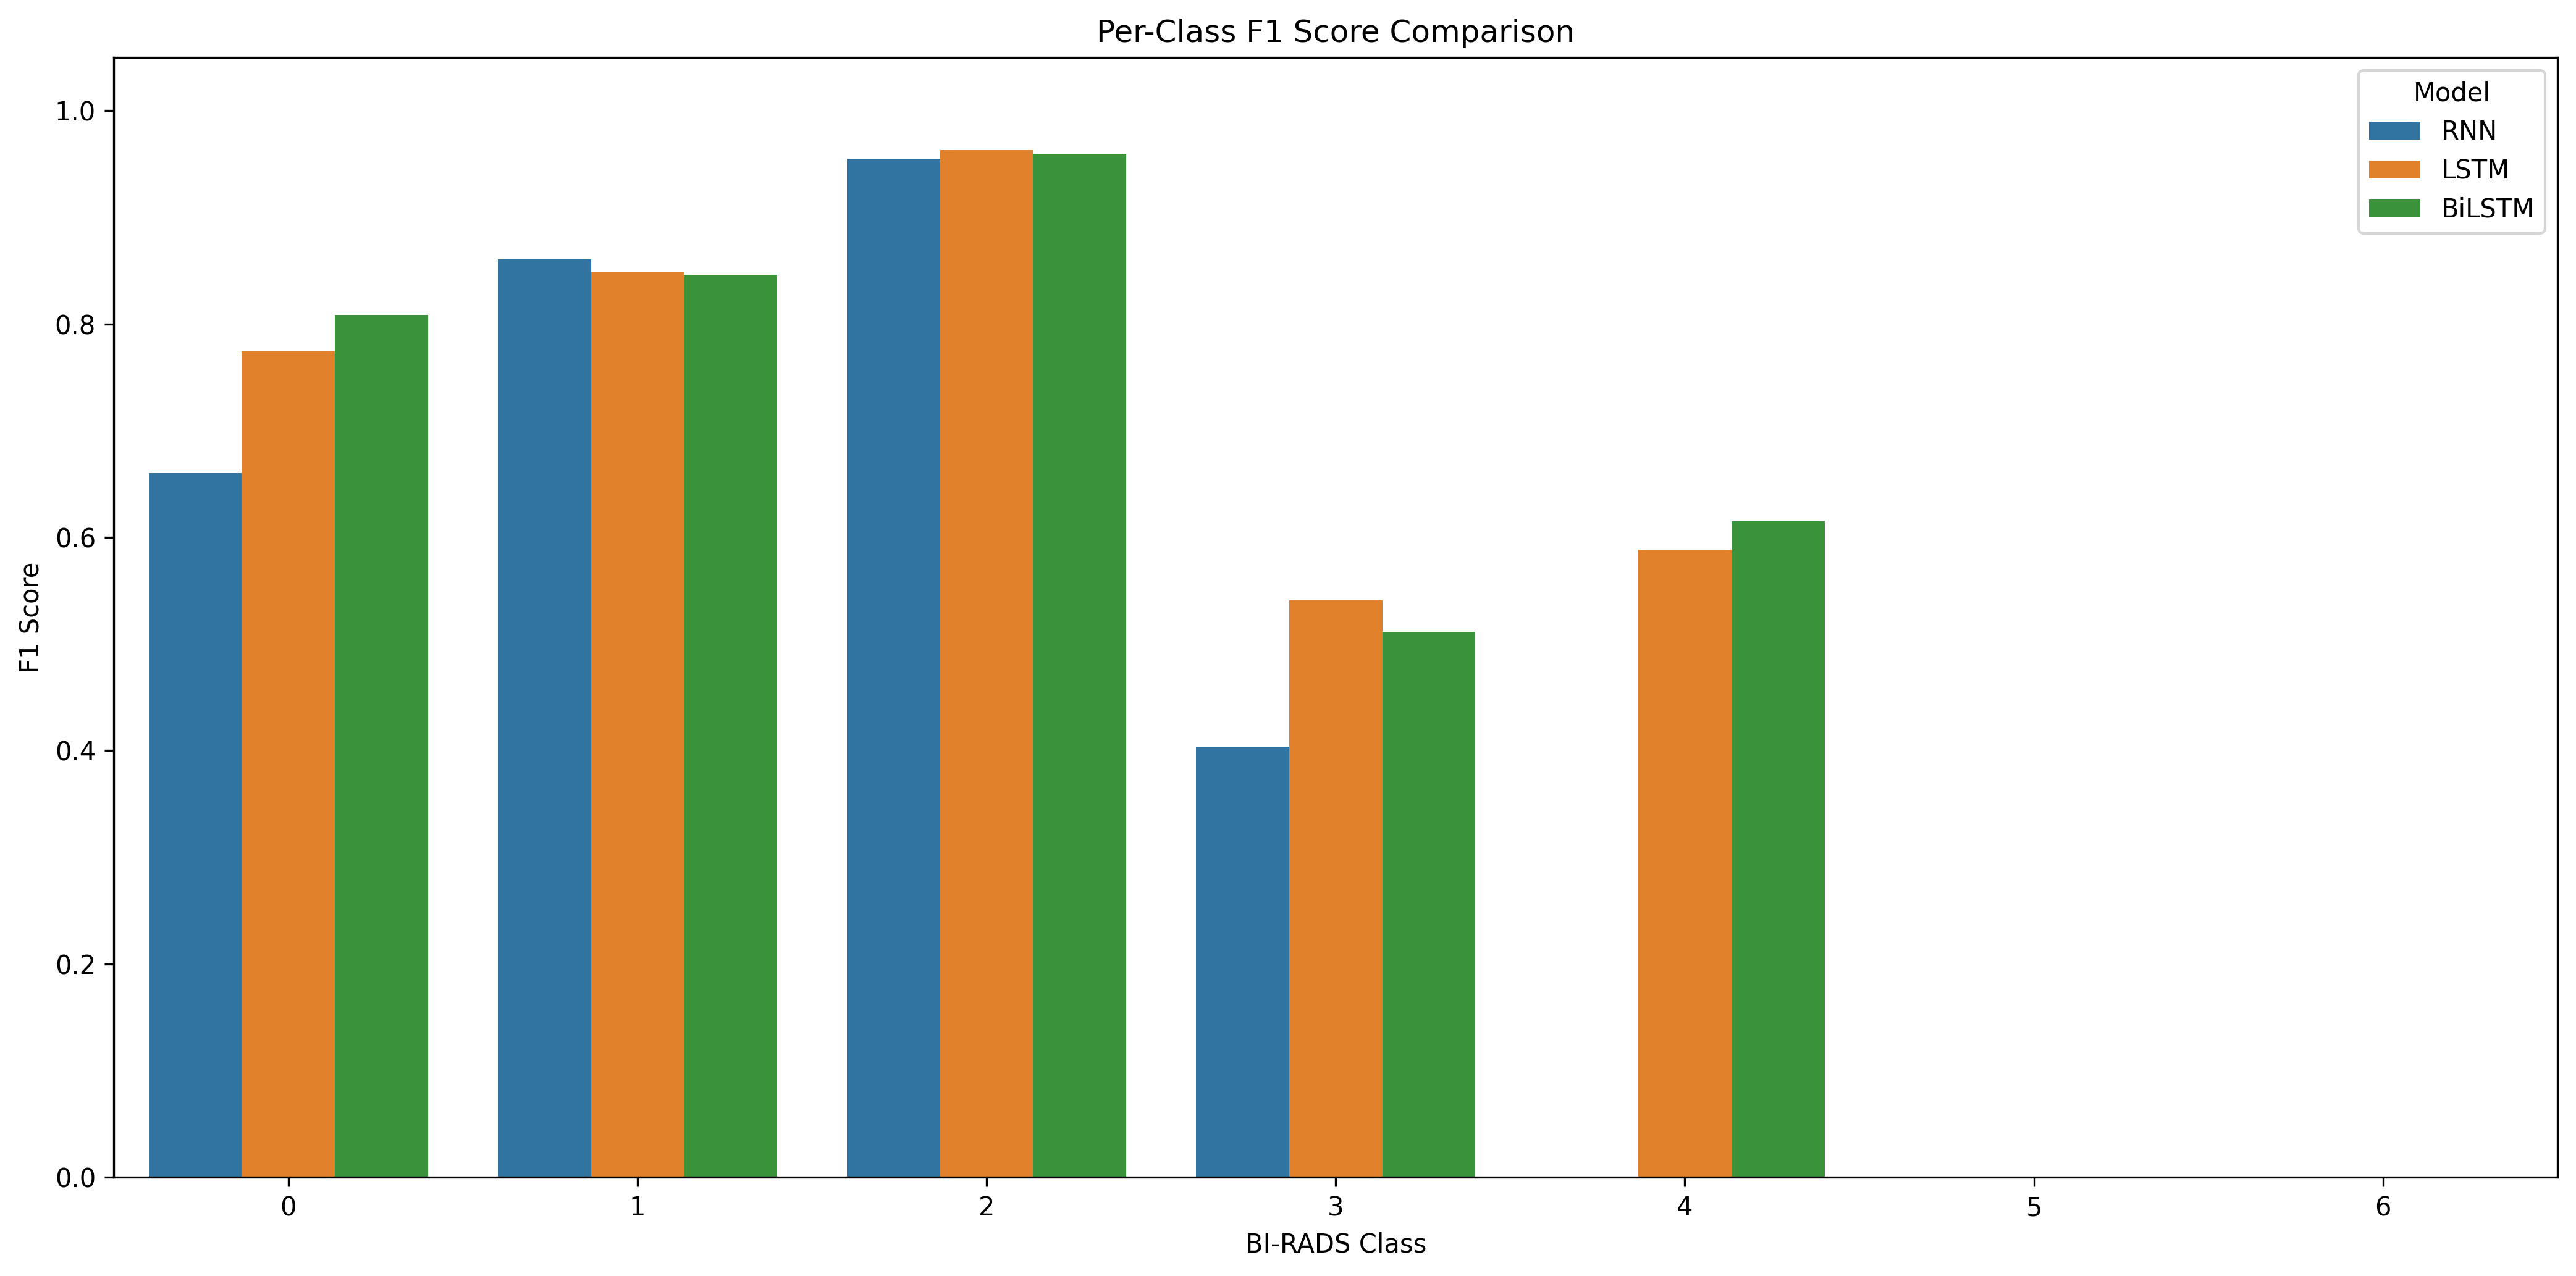
\includegraphics[width=\textwidth]{figures/lstm_per_class_f1.png}
\caption{Per-class F1 score comparison across the three recurrent architectures
(RNN, LSTM, BiLSTM) on the held-out test set. The LSTM achieves the highest
F1 for the majority class (Category~2: 0.97) and competitive scores for the
clinically important Categories~3 and~4, while all three models score zero
on the severely underrepresented Categories~5 and~6.}
\label{fig:lstm_per_class_f1}
\end{figure}

\begin{figure}[h!]
\centering
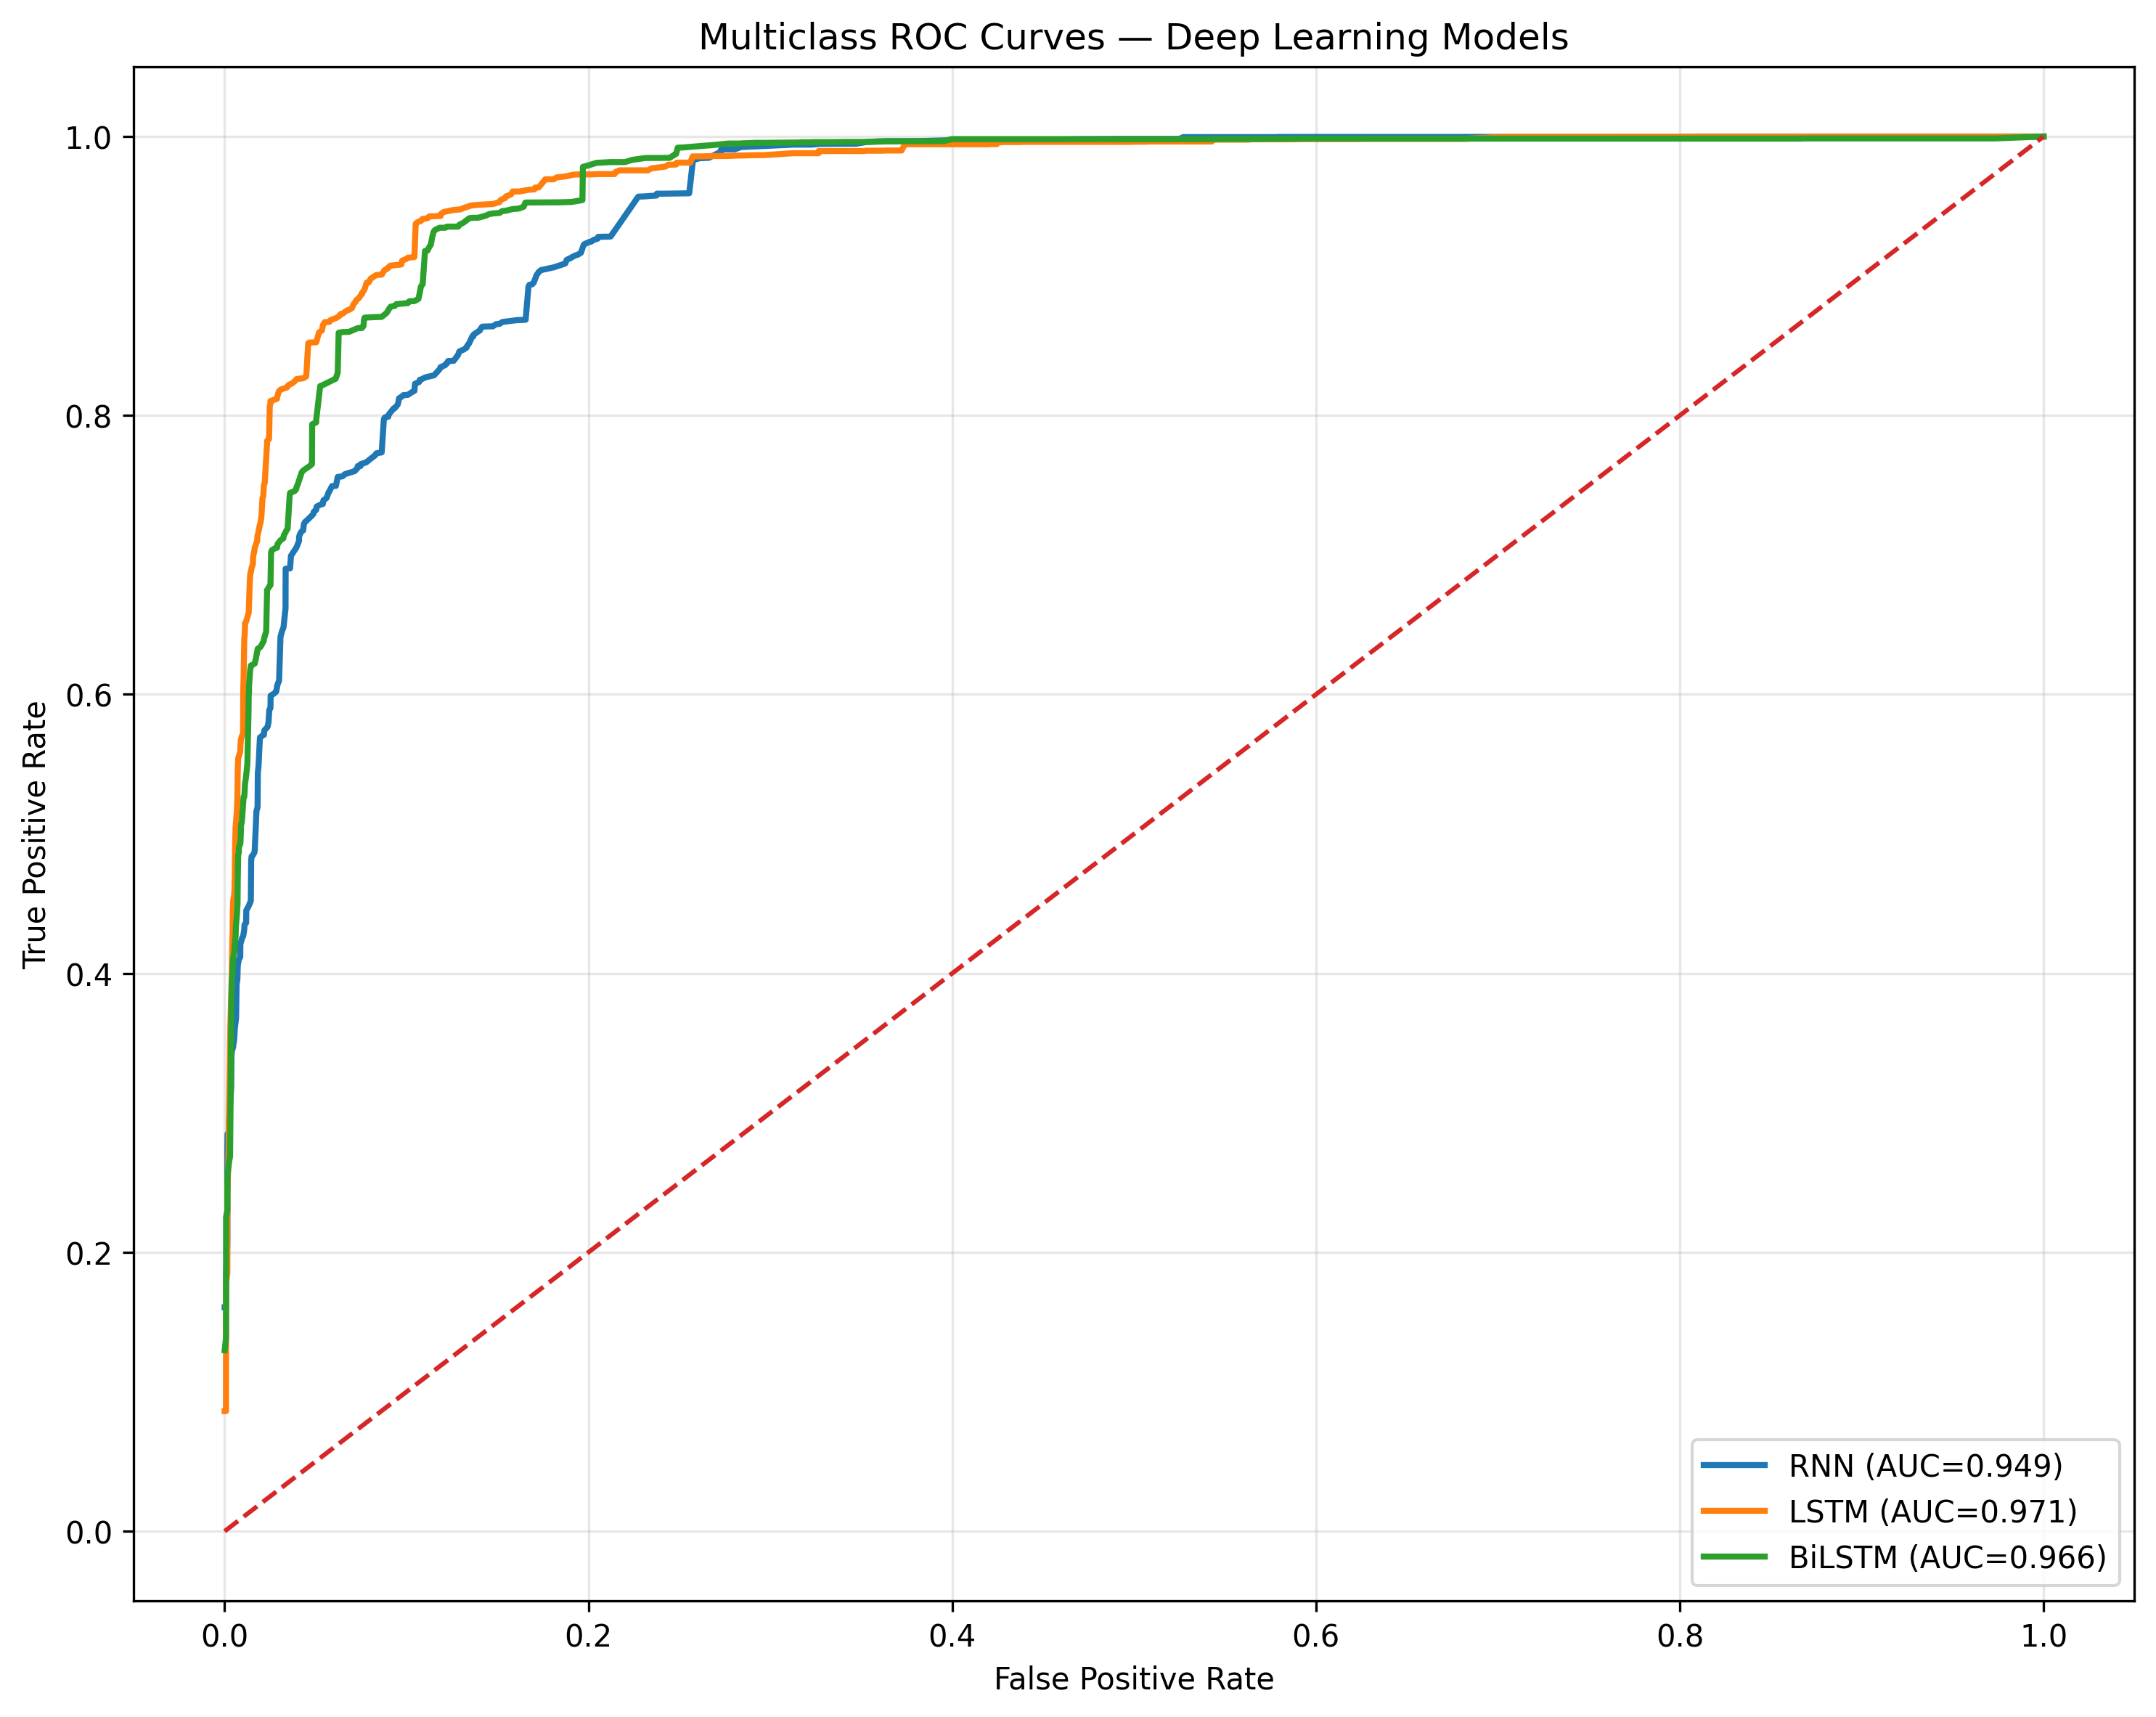
\includegraphics[width=0.85\textwidth]{figures/lstm_roc_curves.png}
\caption{Macro-averaged multiclass ROC curves for the three deep learning
models. The LSTM attains the highest AUC (0.971), confirming that its
posterior probabilities provide strong BI-RADS class discrimination even
for classes where hard classification fails.}
\label{fig:lstm_roc}
\end{figure}

\begin{figure}[h!]
\centering
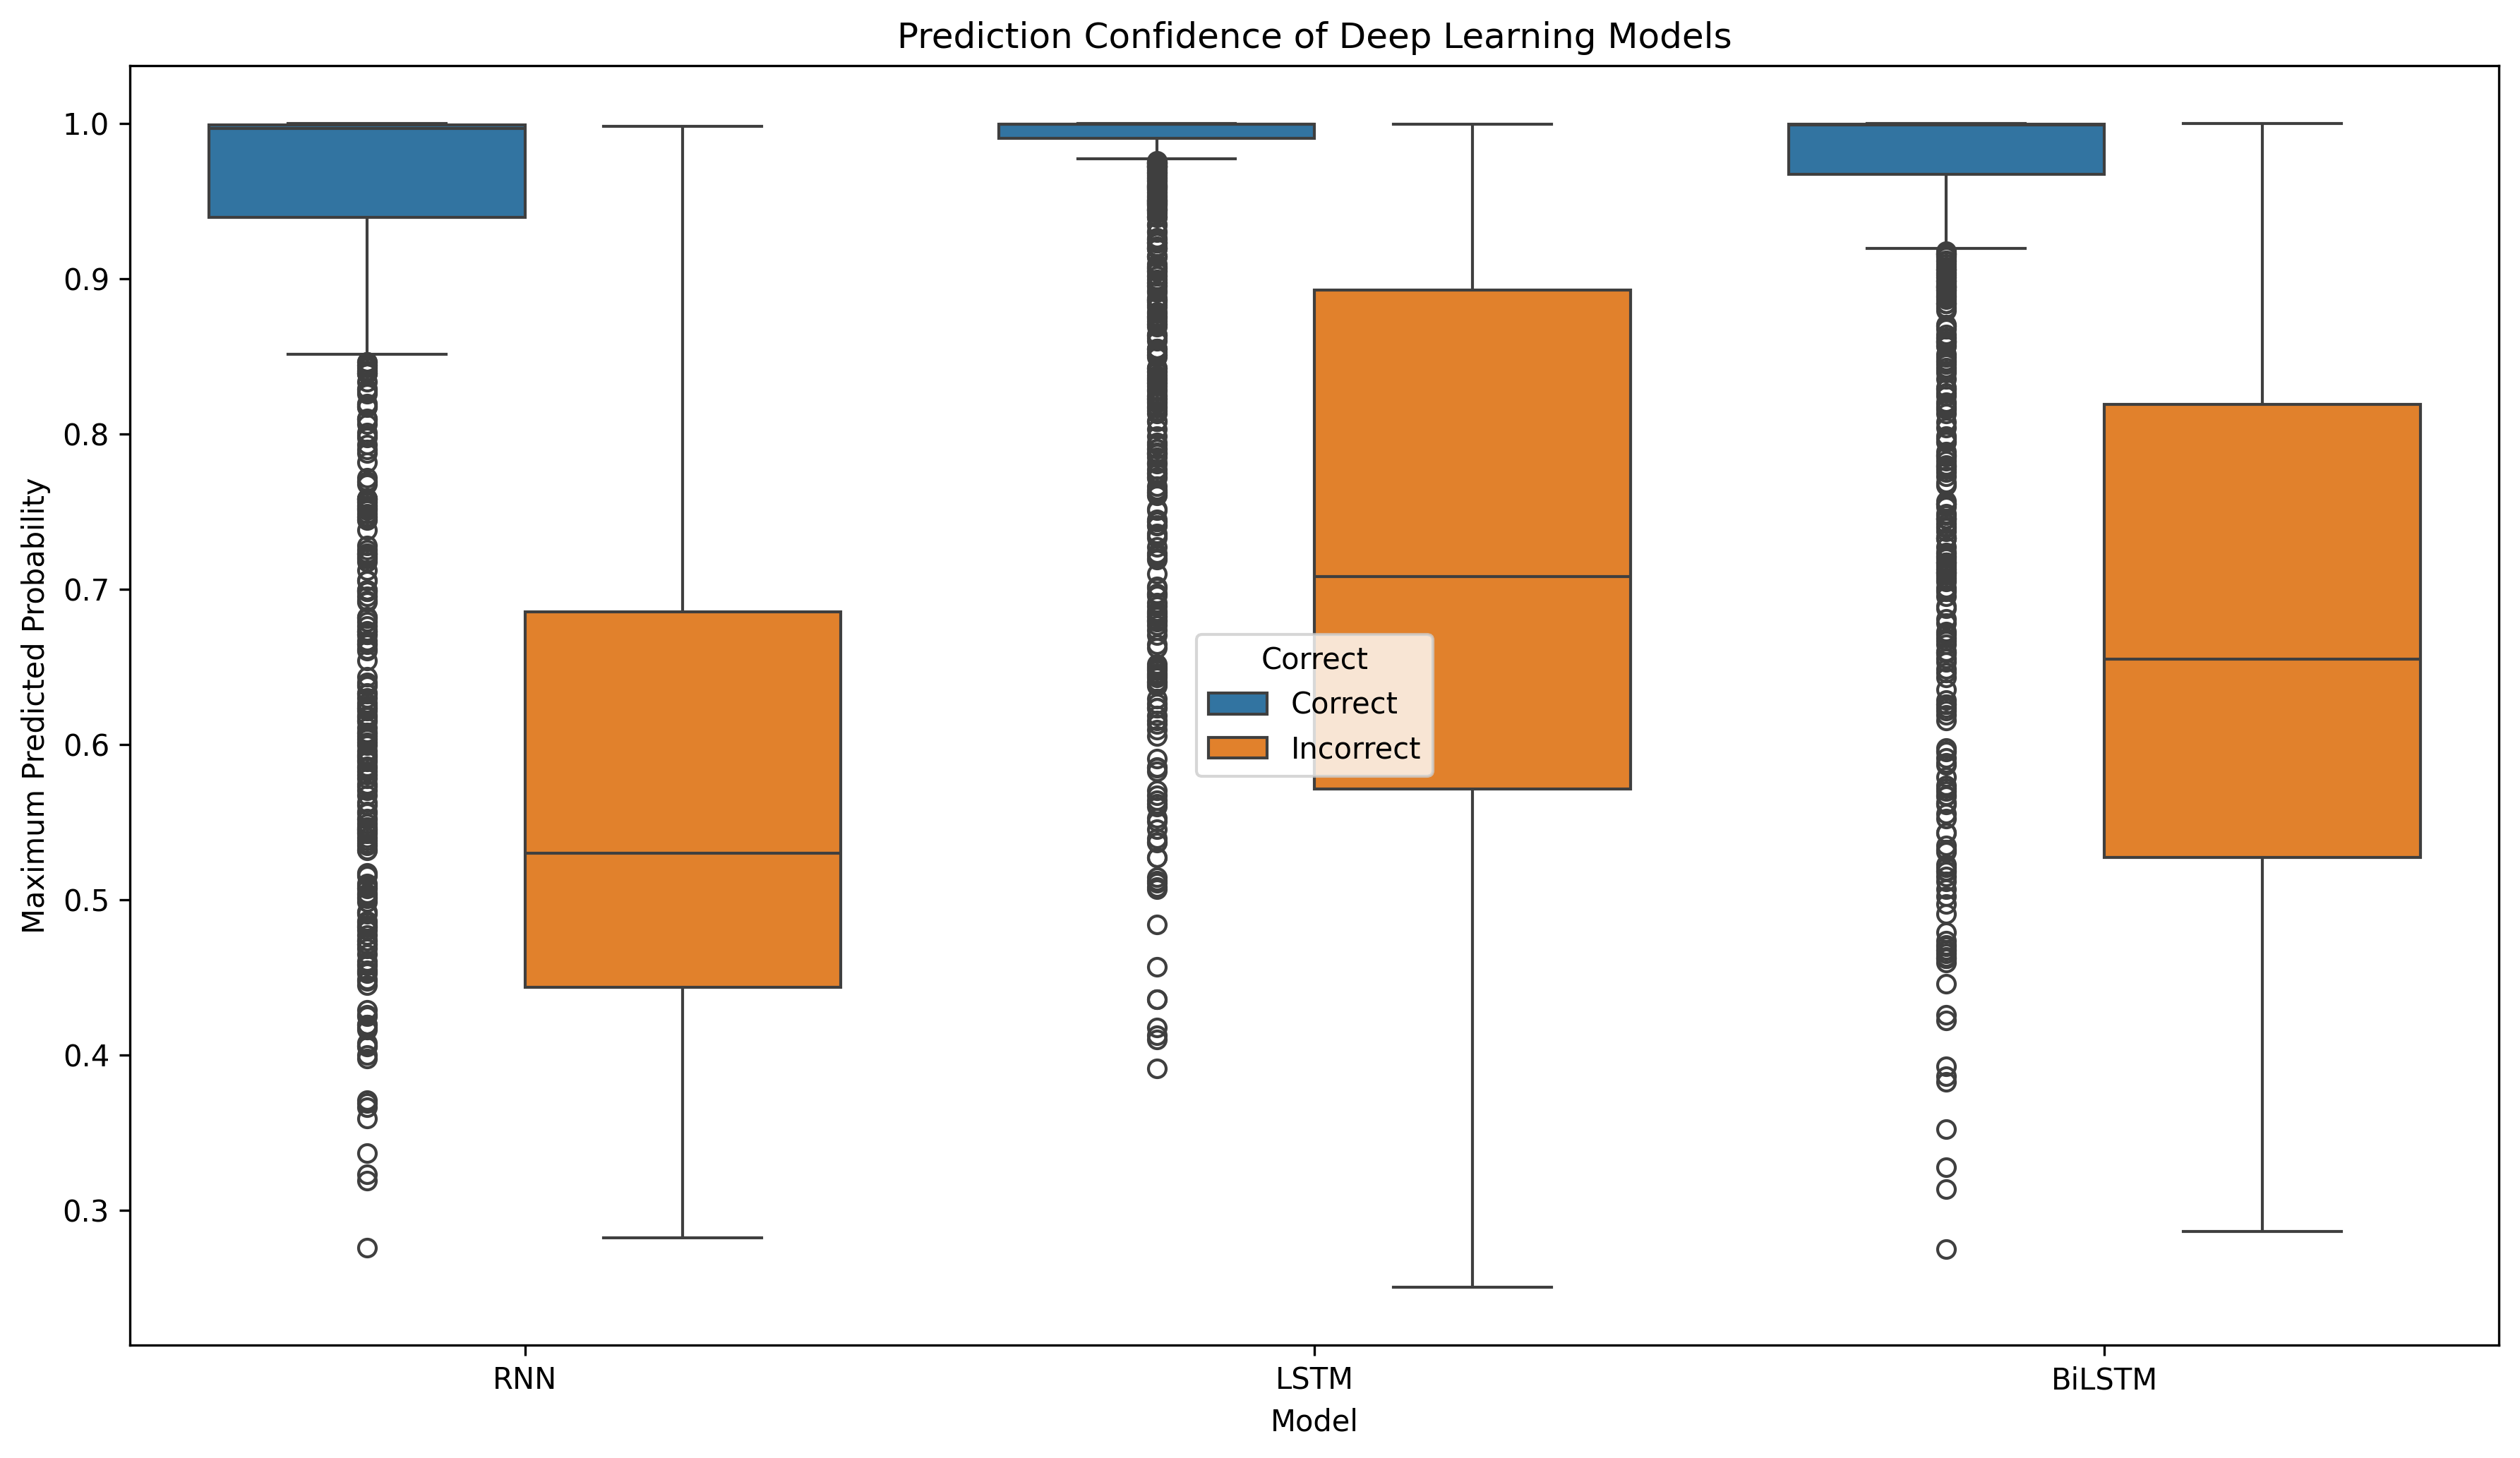
\includegraphics[width=0.9\textwidth]{figures/lstm_prediction_confidence.png}
\caption{Prediction confidence (maximum softmax probability) for correct
vs.\ incorrect predictions across the three deep learning models. The LSTM
shows the clearest separation: correctly classified reports cluster near
probability~1.0, while incorrectly classified reports have a substantially
wider spread, suggesting that the LSTM's confidence score is a usable
proxy for prediction reliability.}
\label{fig:lstm_confidence}
\end{figure}

\textbf{Putting the three families side by side from a clinical perspective.}
For a mammography screening programme, the choice between model families
depends critically on which BI-RADS errors the programme can tolerate.
Classical discriminative classifiers---and especially the linear SVM with
TF-IDF features---maximise weighted F1, which is dominated by Category~2
performance and reflects aggregate accuracy on the bulk of screening reports.
This makes them the most defensible choice for high-throughput pre-screening
of a largely benign population (e.g., routine annual screening), where the
vast majority of reports genuinely are Category~2 and the cost of an
individual misclassification is low.
However, Logistic Regression with CountVectorizer achieves a substantially
higher macro F1 (0.718 vs.~0.696 for the SVM), meaning it is better at
identifying the minority BI-RADS categories---the categories that carry the
greatest clinical consequences (Categories~3, 4, 5, 6).
For a programme that needs to minimise missed Category~3/4 reports (which
require follow-up biopsy or imaging), Logistic Regression is the more
clinically appropriate classical choice.
The Kneser-Ney bigram model occupies a distinct niche: at 85.7\% accuracy
and macro F1 of 0.594, it is not competitive with the discriminative models
on raw performance, but it is the only family whose decision process is fully
transparent.
A radiologist or programme administrator can inspect the class-conditional
bigram likelihood tables directly to understand why the model assigned a
particular BI-RADS score, an audit trail that neither the neural nor the
bag-of-words classifiers can easily provide.
For resource-constrained settings---a clinic without GPU infrastructure, or
one that needs to retrain monthly as new reports accrue---the N-gram model's
4.66-second inference time over the full 1{,}377-report test set and its
near-zero retraining cost make it a practically viable baseline.
The deep learning models top the raw accuracy leaderboard (LSTM: 90.3\%) but
post a substantially lower macro F1 than Logistic Regression (0.531 vs.\ 0.718),
confirming that their high accuracy is driven almost entirely by Category~2
correctness rather than by any genuine improvement on the clinically
challenging minority categories.
For the minority categories that matter most in a breast-cancer screening
programme---BI-RADS~4 (biopsy), 5 (urgent biopsy), and 6 (known
malignancy)---the neural models actually offer the weakest coverage, and
their complete failure on Categories~5 and~6 would be unacceptable without
additional safeguards such as class-weighted loss, data augmentation, or
an ensemble with the N-gram model's MAP scores as a calibration signal.

% ============================================================
\section{Conclusion}
% ============================================================

\subsection{Overall Summary}

We set out to benchmark three model families---Kneser-Ney N-gram language
models, classical bag-of-words discriminative classifiers, and recurrent neural
networks---on automatic BI-RADS category assignment from machine-translated
Portuguese mammography reports.
The central challenge is the severe class imbalance inherent in breast screening
data: BI-RADS~2 (benign, no action) dominates at 80\%+ of reports, while
BI-RADS~5 (highly suggestive of malignancy) and~6 (known biopsy-proven
malignancy)---the categories with the highest clinical urgency---contribute
fewer than 40 training examples combined.
Our domain-aware preprocessing pipeline was designed around this clinical
reality: preserving negation cues (``no mass'', ``without calcification''),
measurement expressions (``2.5~cm'', ``3$\times$2~cm''), and laterality terms
(``right breast'', ``bilateral'') that carry direct BI-RADS-discriminative
information, while removing explicit BI-RADS label leakage to ensure the
models learn report language rather than transcribed category numbers.

No single model dominates across all clinically relevant metrics.
LSTM achieves the highest raw accuracy (90.27\%), but this is largely driven
by near-perfect classification of the dominant BI-RADS~2 class.
TF-IDF with a Linear SVM achieves the highest weighted F1 (89.99\%), again
reflecting its strength on the majority class.
CountVectorizer with Logistic Regression achieves the highest macro F1
(71.8\%), indicating the best balance across all seven BI-RADS categories
including the minority ones.
For a breast screening programme where missing a Category~4, 5, or~6 report
has the most serious patient-safety consequences, macro F1 is the most
clinically meaningful single-number summary---and by this metric, a
well-regularised linear model outperforms both the N-gram and deep learning
families.
The Kneser-Ney bigram, meanwhile, held its own as a transparent and deployable
baseline: 85.7\% accuracy and 59.4\% macro F1, with the ability to flag
some Category~5 and~6 reports (which no deep learning model ever predicts),
and full interpretability of the class-conditional language statistics
that drive each prediction.

\subsection{Pros}
\label{sec:strengths}

From a clinical deployment perspective, several strengths are worth
highlighting.
First, the domain-aware preprocessing pipeline---which preserves negation
cues, measurement spans, laterality terms, and clinical abbreviations while
excising BI-RADS label leakage---ensures that models learn genuine radiological
language patterns rather than trivially regressing on leaked category labels.
The SHAP and LIME explainability analyses confirm this: the tokens with the
highest attribution scores (``spiculated'', ``irregular'', ``no dominant mass'',
``bilateral'') are precisely the terms that the ACR BI-RADS Atlas identifies
as category-discriminative descriptors.
Second, all three model families are evaluated on the same stratified
70/15/15 split, enabling a fair head-to-head comparison that is often absent
in the clinical NLP literature, where different studies evaluate different
datasets with different protocols.
Third, the Kneser-Ney bigram's class-conditional log-posteriors are fully
transparent: a radiologist, clinical informaticist, or programme auditor can
inspect which word pairs the model associates with each BI-RADS category,
an audit trail of direct clinical relevance that neither the neural nor the
bag-of-words models provide as naturally.
Fourth, the LSTM's prediction confidence scores (maximum softmax probability)
are well-calibrated enough to identify uncertain borderline reports
(confidence $<$ 0.95) that would benefit most from radiologist review,
potentially enabling a human-in-the-loop triage workflow that concentrates
expert attention on the cases where the model is least sure.
Among the classical models, Logistic Regression with balanced class weights
provides the best minority-class coverage (macro F1 = 0.718) without GPU
infrastructure, making it a viable option for lower-resource breast-screening
programmes.

\subsection{Limitations}

Several limitations temper these results.
Class imbalance is the most clinically consequential: BI-RADS~5 and~6 together
contribute only 52 of the 9{,}179 unique reports (0.57\%), with 20 and 32
training examples respectively.
This is a fundamental data problem for breast-screening corpora, where
malignant findings are rare by design, and it directly causes all three deep
learning architectures to produce zero predictions for both categories---the
most clinically dangerous failure mode possible.
Oversampling, focal loss, or synthetic data augmentation targeted specifically
at BI-RADS~4, 5, and~6 reports would be the highest-priority fix for any
deployment-oriented follow-up.
Translation quality is a second open issue: automated Portuguese-to-English
translation may subtly alter or lose clinical modifiers (e.g., hedging adverbs,
degree terms such as ``slightly'', ``markedly''), introduce false negations, or
mistranslate measurement units and anatomical directions, any of which could
corrupt the BI-RADS-discriminative signal that models rely on.
The quality assessment was limited to a spot-check of 50 reports rather than a
systematic error-type audit, so the extent of translation-induced noise remains
unquantified.
A degree of residual label leakage also remains: 181 reports still contain
partial BI-RADS cue fragments after cleaning, which may inflate performance
estimates for models that are sensitive to those fragments.
No transformer-based clinical language models (ClinicalBERT~\cite{alsentzer2019publicly},
BioBERT, or Portuguese-specific BERT variants) were evaluated in this study,
so the performance gap between recurrent architectures and the current state
of the art in clinical NLP remains uncharted for this corpus.
Finally, the translate-then-classify paradigm has been validated only for the
Portuguese$\to$English direction on this specific dataset; the
translate-test literature~\cite{artetxe2023revisiting,papaioannou2022cross}
suggests that performance can vary substantially across language pairs and
translation systems, particularly for low-resource clinical domains where
translation models may not be fine-tuned on radiology text.

% ============================================================
\section{Future Scope}
% ============================================================

A number of directions could extend this work. One is transformer
fine-tuning: fine-tuning ClinicalBERT~\cite{alsentzer2019publicly}, BioBERT,
or a Portuguese clinical BERT directly on the original Portuguese text,
rather than on translated English. Related to this is the possibility of
multilingual models, applying mBERT or XLM-R to raw Portuguese reports to
eliminate translation noise altogether, in the spirit of the cross-lingual
transfer strategies studied by Papaioannou et al.~\cite{papaioannou2022cross}
and the translate-test analysis of Artetxe et al.~\cite{artetxe2023revisiting}.
Class imbalance mitigation is another natural next step, whether through
oversampling with SMOTE~\cite{chawla2002smote}, focal
loss~\cite{lin2017focal}, or data augmentation targeted at the minority
BI-RADS categories (4, 5, 6). A further avenue is an N-gram plus ML ensemble
that combines MAP log-posterior scores from the N-gram model with TF-IDF
features as input to a meta-classifier. Building on the SHAP and LIME
explainability analyses conducted for the LSTM in this work, a natural next
step is to extend token-level attribution to all model families and to
aggregate attributions across the full test set to produce class-level feature
importance rankings, while temporal validation could evaluate robustness
across different acquisition years, hospitals, and radiologist writing
styles. Finally, multi-modal integration could combine report text with
image-derived mammographic features, in the spirit of image-based
mammography models such as~\cite{yala2019deep}, within a single joint
model.

% ============================================================
%  References
%  Every entry below is fully wrapped in \href{URL}{...} (via hyperref),
%  so clicking the citation text itself opens the source -- the raw URL
%  is not printed. Every entry is cited at least once in the body text above.
% ============================================================
\begin{thebibliography}{99}

\bibitem{acr2013}
\href{https://www.acr.org/Clinical-Resources/Clinical-Tools-and-Reference/Reporting-and-Data-Systems/Bi-Rads}{%
American College of Radiology (ACR).
\textit{ACR BI-RADS Atlas, Breast Imaging Reporting and Data System}, 5th~ed.
ACR, Reston, VA, 2013.}

\bibitem{kneser1995improved}
\href{https://ieeexplore.ieee.org/document/479394}{%
R.~Kneser and H.~Ney.
Improved backing-off for M-gram language modeling.
In \textit{Proc.\ IEEE ICASSP}, pp.~181--184, 1995.}

\bibitem{hochreiter1997long}
\href{https://doi.org/10.1162/neco.1997.9.8.1735}{%
S.~Hochreiter and J.~Schmidhuber.
Long short-term memory.
\textit{Neural Computation}, 9(8):1735--1780, 1997.}

\bibitem{schuster1997bidirectional}
\href{https://doi.org/10.1109/78.650093}{%
M.~Schuster and K.~K.~Paliwal.
Bidirectional recurrent neural networks.
\textit{IEEE Trans.\ Signal Processing}, 45(11):2673--2681, 1997.}

\bibitem{hassanpour2017information}
\href{https://doi.org/10.1016/j.artmed.2015.09.007}{%
S.~Hassanpour and C.~P.~Langlotz.
Information extraction from multi-institutional radiology reports.
\textit{Artificial Intelligence in Medicine}, 66:29--39, 2016.}

\bibitem{yala2019deep}
\href{https://doi.org/10.1148/radiol.2019182716}{%
A.~Yala, C.~Lehman, T.~Schuster, T.~Portnoi, and R.~Barzilay.
A deep learning mammography-based model for improved breast cancer risk prediction.
\textit{Radiology}, 292(1):60--66, 2019.}

\bibitem{peng2018negbio}
\href{https://pmc.ncbi.nlm.nih.gov/articles/PMC5961815/}{%
Y.~Peng, X.~Wang, L.~Lu, M.~Bagheri, R.~Summers, and Z.~Lu.
NegBio: a high-performance tool for negation and uncertainty detection in radiology reports.
\textit{AMIA Summits on Translational Science Proceedings}, pp.~188--196, 2018.}

\bibitem{friedman2004natural}
\href{https://doi.org/10.1197/jamia.M1552}{%
C.~Friedman, L.~Shagina, Y.~Lussier, and G.~Hripcsak.
Automated encoding of clinical documents based on natural language processing.
\textit{Journal of the American Medical Informatics Association}, 11(5):392--402, 2004.}

\bibitem{chen1998evaluation}
\href{https://doi.org/10.1006/csla.1999.0128}{%
S.~F.~Chen and J.~Goodman.
An empirical study of smoothing techniques for language modeling.
\textit{Computer Speech \& Language}, 13(4):359--394, 1999.}

\bibitem{alsentzer2019publicly}
\href{https://aclanthology.org/W19-1909/}{%
E.~Alsentzer, J.~R.~Murphy, W.~Boag, W.-H.~Weng, D.~Jindi, T.~Naumann, and M.~McDermott.
Publicly available clinical BERT embeddings.
In \textit{Proc.\ 2nd Clinical NLP Workshop}, 2019.}

\bibitem{nassif2012extracting}
\href{https://pmc.ncbi.nlm.nih.gov/articles/PMC3688645}{%
H.~Nassif, F.~Cunha, I.~C.~Moreira, R.~Cruz-Correia, E.~Sousa, D.~Page, E.~Burnside, and I.~Dutra.
Extracting BI-RADS features from Portuguese clinical texts.
In \textit{IEEE Int.\ Conf.\ on Bioinformatics and Biomedicine (BIBM)}, pp.~1--4, 2012.}

\bibitem{joachims1998text}
\href{https://link.springer.com/chapter/10.1007/BFb0026683}{%
T.~Joachims.
Text categorization with support vector machines: learning with many relevant features.
In \textit{Proc.\ 10th European Conference on Machine Learning (ECML)}, 1998.}

\bibitem{salton1988term}
\href{https://doi.org/10.1016/0306-4573(88)90021-0}{%
G.~Salton and C.~Buckley.
Term-weighting approaches in automatic text retrieval.
\textit{Information Processing \& Management}, 24(5):513--523, 1988.}

\bibitem{mccallum1998naive}
\href{https://www.cs.cmu.edu/~knigam/papers/multinomial-aaaiws98.pdf}{%
A.~McCallum and K.~Nigam.
A comparison of event models for Naive Bayes text classification.
In \textit{AAAI-98 Workshop on Learning for Text Categorization}, pp.~41--48, 1998.}

\bibitem{breiman2001random}
\href{https://doi.org/10.1023/A:1010933404324}{%
L.~Breiman.
Random forests.
\textit{Machine Learning}, 45:5--32, 2001.}

\bibitem{chen2016xgboost}
\href{https://doi.org/10.1145/2939672.2939785}{%
T.~Chen and C.~Guestrin.
XGBoost: a scalable tree boosting system.
In \textit{Proc.\ 22nd ACM SIGKDD International Conference on Knowledge Discovery and Data Mining},
pp.~785--794, 2016.}

\bibitem{karimi2017automatic}
\href{https://aclanthology.org/W17-2342/}{%
S.~Karimi, X.~Dai, H.~Hassanzadeh, and A.~Nguyen.
Automatic diagnosis coding of radiology reports: a comparison of deep learning and conventional classification methods.
In \textit{Proc.\ BioNLP 2017 Workshop}, pp.~328--332, 2017.}

\bibitem{mikolov2013efficient}
\href{https://arxiv.org/abs/1301.3781}{%
T.~Mikolov, K.~Chen, G.~Corrado, and J.~Dean.
Efficient estimation of word representations in vector space.
In \textit{International Conference on Learning Representations (ICLR)}, 2013.}

\bibitem{pennington2014glove}
\href{https://doi.org/10.3115/v1/D14-1162}{%
J.~Pennington, R.~Socher, and C.~D.~Manning.
GloVe: global vectors for word representation.
In \textit{Proc.\ 2014 Conference on Empirical Methods in Natural Language Processing (EMNLP)},
pp.~1532--1543, 2014.}

\bibitem{artetxe2023revisiting}
\href{https://aclanthology.org/2023.emnlp-main.399/}{%
M.~Artetxe, V.~Goswami, S.~Bhosale, A.~Fan, and L.~Zettlemoyer.
Revisiting machine translation for cross-lingual classification.
In \textit{Proc.\ 2023 Conference on Empirical Methods in Natural Language Processing},
pp.~6489--6499, 2023.}

\bibitem{papaioannou2022cross}
\href{https://aclanthology.org/2022.lrec-1.95/}{%
J.-M.~Papaioannou, P.~Grundmann, B.~van Aken, A.~Samaras, I.~Kyparissidis,
G.~Giannakoulas, F.~Gers, and A.~L\"oser.
Cross-lingual knowledge transfer for clinical phenotyping.
In \textit{Proc.\ 13th International Conference on Language Resources and Evaluation (LREC)},
pp.~900--909, 2022.}

\bibitem{chawla2002smote}
\href{https://doi.org/10.1613/jair.953}{%
N.~V.~Chawla, K.~W.~Bowyer, L.~O.~Hall, and W.~P.~Kegelmeyer.
SMOTE: synthetic minority over-sampling technique.
\textit{Journal of Artificial Intelligence Research}, 16:321--357, 2002.}

\bibitem{lin2017focal}
\href{https://doi.org/10.1109/ICCV.2017.324}{%
T.-Y.~Lin, P.~Goyal, R.~Girshick, K.~He, and P.~Doll\'{a}r.
Focal loss for dense object detection.
In \textit{Proc.\ IEEE International Conference on Computer Vision (ICCV)},
pp.~2980--2988, 2017.}

\bibitem{saito2015precision}
\href{https://doi.org/10.1371/journal.pone.0118432}{%
T.~Saito and M.~Rehmsmeier.
The precision-recall plot is more informative than the ROC plot when evaluating binary classifiers on imbalanced datasets.
\textit{PLOS ONE}, 10(3):e0118432, 2015.}

\bibitem{sokolova2009systematic}
\href{https://doi.org/10.1016/j.ipm.2009.03.002}{%
M.~Sokolova and G.~Lapalme.
A systematic analysis of performance measures for classification tasks.
\textit{Information Processing \& Management}, 45(4):427--437, 2009.}

\end{thebibliography}

\end{document}